\documentclass{article}

\usepackage[right=1in,left=1in,top=1in,bottom=1in]{geometry}

\usepackage{mhchem}

\usepackage{xcolor}

\usepackage{blkarray}

\usepackage{amsmath}

\usepackage{amsfonts}

\usepackage{tikz}
\usetikzlibrary{shapes.geometric, arrows}
\usetikzlibrary{arrows, decorations.markings}
\usetikzlibrary{positioning}

\tikzstyle{startstop} = [rectangle, rounded corners, minimum width=3cm, minimum height=1.0cm, text centered, draw=black, fill=lightgray]
\tikzstyle{process} = [rectangle, minimum width=6cm, minimum height=1.0cm, text width = 5cm, text centered, draw=black, fill=lightgray]
\tikzstyle{decision} = [diamond, minimum width=2cm, minimum height=1cm, text width = 3cm, text centered, draw=black, fill=lightgray]
\tikzstyle{io} = [trapezium, trapezium left angle=70, trapezium right angle=110, minimum width=3cm, text width = 3cm, minimum height=1cm, text centered, draw=black, fill=lightgray]
\tikzstyle{arrow} = [thick,->,>=stealth]

\usepackage{amsmath}

\numberwithin{equation}{section}

\usepackage{listings}

%Create the color for the code background
\definecolor{light-gray}{gray}{0.85}

% This makes a listing environment for input templates 

\lstnewenvironment{lt}
{
    \lstset{
        basicstyle=\ttfamily,
        backgroundcolor=\color{light-gray},
        emph={action, ader_neg_adens, ader_trans_iter, burn, cnd, cnt, cont, control, conditions, dir, disc, feed, feed_and_remv, form, frac, from, group, grp, grp2, isos, keyword, kmax, kmin, mass, mat, max, min, mols, omp, opt, oxi, oxidation, pres, prop, reac, redox, rem, remv, rhow, rng, rto, set, spec_stream, stream, streams, sum, to, transfers, type, val, vol, weight},
        emphstyle=\underbar,
    }
}{}

% This makes a listing environment for input examples
\lstnewenvironment{li}
{
    \lstset{
        basicstyle=\bfseries\color{white},
        backgroundcolor=\color{black},
    }
}{}

\begin{document}

\title{ADER: Advanced Depletion Extension for Reprocessing\\
\vspace{10pt}\large{Ver: 1.0 - A SERPENT2 Extension}\\
\vspace{10pt}\large{User Manual}}

\author{
    Daniel D. Wooten
}

\clearpage
\maketitle
\pagebreak
\tableofcontents
\pagebreak

\section{Preface}\label{sec:pref}
This document is intended for users of SERPENT2 wishing to utilize the
\textbf{A}dvanced \textbf{D}epletion \textbf{E}Extension for
\textbf{R}eprocessing ( ADER ) extension.
\textbf{This manual assumes the reader is proficient with SERPENT2.}
General information about SERPENT2 can be found at the SERPENT2
wiki: 
\begin{lstlisting}[breaklines, backgroundcolor=\color{white}]{website}
serpent.vtt.ft/mediawiki/index.php/Main_Page
\end{lstlisting}

With regards to citing SERPENT2 and ADER, as stated on the SERPENT2 wiki general
reference to SERPENT2 may be provided by - J. Leppanen, M. Pusa, T. Vittanen,
V. Valtavirta, T. Kaltiaisenaho. \textit{``The Serpent Monte Carlo code: Status,
development, and applications in 2013"}. Ann. Nucl. Energy, \textbf{82} (2015)
142 - 150. Reference to ADER may be provided by - D. D. Wooten. \textit{ADER -
Advanced Depletion Extension for Reprocessing}. (2019).

ADER makes extensive use of the open-source library, Clp, part of the COIN-OR
collection of packages. Supporting documentation and the source code
for Clp can be found at: 
\begin{lstlisting}[breaklines, backgroundcolor=\color{white}]{website}
https://github.com/coin-or/Clp
\end{lstlisting}
Of importance is that Clp is distributed under
the Eclipse Public Licence which is not a copy-left licence but a rather
forgiving open-source licence. Instructions for installing and linking the
Clp libraries can be found in section \ref{sec:install}.

\noindent Examples of SERPENT2 input are given 
\begin{lt}
in this font
\end{lt}
SERPENT2 and ADER keywords, user inputs which must be a certain word, 
appear underlined as seen below. \textbf{Keywords not enclosed in brackets
must appear in the position of the entry they are seen in. Keywords enclosed in
brackets may appear anywhere after this opening keyword but must be followed
by their input value if they have one.}
\begin{lt}
keyword
\end{lt}
The following list of symbols are not to be considered ``input". Rather, they
are delimiters for this manual and should not be considered part of any ADER
commands or inputs\ldots
\begin{lt}
[ ] { } < > ( ) ; ...
\end{lt}
Required user inputs are denoted\ldots
\begin{lt}
[This_entry_is_set_by_the_user]
\end{lt}
Optional user inputs are denoted\ldots 
\begin{lt}
<This_entry_may_be_excluded>
\end{lt}
Required user choices from a list are denoted\ldots
\begin{lt}
[{option_1; option_2}]
\end{lt}
Optional user choices from a list are denoted\ldots
\begin{lt} 
<{option_1; option_2}>
\end{lt}
User inputs which are required \textit{if} a previous input was given are 
denoted\ldots
\begin{lt}
<optional_input> (required_input_due_to_earlier_input)
\end{lt}
If an example of a user input includes a structure such as\ldots
\begin{lt}
[Entry_1] [some_number]
...
<Entry_n> (some_number)
\end{lt}
This indicates that at least one instance of \texttt{Entry x} must be input by
the user but as many instances of type \texttt{Entry x} may be input by the
user. Additionally the presence of the second bracketed input indicates that
each instance of \texttt{Entry x} requires an entry of \texttt{some\_number}.
Examples of generic SERPENT2 input, input templates, are given in a light-gray
box with black mono-spaced font such as the example seen below\ldots

\begin{lt}
mat [mat_name] [mat_den] <{vol,mass}> [mat_val] <burn> (burn_segments) 
[isotope_1_zai].[temp_lib] [iso_frac]
<isotope_n_zai>.(temp_lib) (iso_frac)
\end{lt}

While any specific use examples, implementations of SERPENT2 input, are given
in a black box with white mono-spaced font such as the example seen below\ldots

\begin{li}
mat water -1.0 vol 1.0 burn 0.0
1001.06c    2
...
1608.06c    1
\end{li}

\section{Introduction}\label{sec:intro}

\textit{Please be sure to read the preface for important information.}\\
In the most direct sense ADER seeks to accomplish two tasks: 
determining an  optimal  material  composition  given  a  set  
of  constraints,  and  integrating the necessary composition adjustments 
into a nuclear material evolution model.
ADER brings to Serpent 2 the ability to define groups of elements,
isotopes, and chemicals; the ability to define relationships between these 
groups; and the ability to move these groups into, out-of, and between 
materials. Furthermore, ADER provides the ability to set
$k_{eff}$ targets, to prescribe mass transfers within a given system, and to set
weighted oxidation state targets for materials. Bringing all of these
capabilities together ADER employs the COIN-OR linear optimization (CLP) 
package to determine the material flows, as  set by the user, 
that will best satisfy an optimization target, also set by the user. 
Sufficiently simplified - ADER is a material-composition, linear-optimization
engine for the SERPENT2 burnup routines. 

This manual serves as both a reference for the theory of ADER and as a guide to
its usage. As such each section has a ``Quick Reference" subsection where
direct and simplified answers to common usage questions and input formatting
can be found. However, many users will find that a deeper understanding of the
theory behind ADER, as well as the nuances of its use, will serve them well. 
This manual is organized to be red through in a linear fashion by a first time
user beginning with the concept of a ``group" as it is used in ADER and
building up the ADER toolkit from there.

To provide context for the explanation of the components of ADER components of
an example simulation are built up throughout this manual. These components only
serve as rough examples.
That said, for this example consider a fuel salt for
a liquid fuel molten salt reactor composed of \ce{LiF} salt at 71.7
mol-fraction, \ce{BeF2} salt at 16 mol-fraction,
\ce{UF3} at 0.023 mol-fraction, \ce{UF4} at 2.277 mol-fraction, 
and \ce{ThF4} at 10 mol-fraction. Take this salt to have
an initial neutron multiplication factor of $1.0$ ( it does not in reality )
and to be in an infinite lattice with a graphite moderator which takes up 50\%
of the volume. The SERPENT2 material based off this example is shown below.
\textbf{The keyword ``ader" must be included in the definition line of any 
material which is to be managed by the ADER extensions to SERPENT2 - i.e. the
material is either connected to a stream or to a conditions block.} ADER input
is entered as a ``regular" component of SERPENT2 input files.

\begin{li}
mat FuelSalt -2.805 vol 1 burn 0 ader
3006.06c    0.00028
3007.06c    0.28323
4009.06c    0.06328
9019.06c    0.60450
90232.06c   0.03954
92233.06c   0.00046
92238.06c   0.00864
\end{li}

\section{Groups}\label{sec:groups}
At the most fundamental level a group in ADER is a list of proportions. This
list describes the relative proportions of elements within the group. These
elements may or may not have specified isotopic proportions and elements
without a specified isotopic composition are permitted in the same group as
elements \textit{with} a specified isotopic composition. Consider a group which
specifies that fluorine be four times as abundant as uranium, within the group.
This group could be used to describe a single molecule of \ce{UF4} or, just as
equivalently, one mol of uranium and four mols of fluorine all in a bucket
on a lab bench. A group is not defined by a quantity of material, but rather
a recipe for a material. Just like defining materials in SERPENT2, the
proportions of an element within a group are normalized to unity and the
proportions of an isotope within an element are normalized to unity.
As such groups in ADER are defined according to four
methods A, B, C, or D as seen bellow.\\

\noindent Method A: 
\begin{lt}
grp [Name] 
[Element_1] [Element_1_frac] 
... 
<Element_n> (Element_n_frac)
\end{lt}

\noindent Method B:
\begin{lt}
grp [Name] 
[Element_1] [Element_1_frac] <isos> (n_isos)
(Iso_1) (Iso_1_frac)
<Iso_n> (Iso_n_frac)
...
<Element_x> [Element_x_frac] <isos> (b_isos)
(Iso_1) (Iso_1_frac)
<Iso_b> (Iso_b_frac)
\end{lt}

\noindent Method C:
\begin{lt}
grp [Name] 
[Element_1] [Element_1_frac] 
...
<Element_x> [Element_x_frac] <isos> (b_isos)
(Iso_1) (Iso_1_frac)
<Iso_b> (Iso_b_frac)
\end{lt}

\noindent Method D:
\begin{lt}
grp [Name] [sum]
[Name_of_group_1] 1
...
<Name_of_group_n> 1
\end{lt}

The keyword \texttt{grp} begins the group section input. All input following 
this word, until the next keyword is found, is taken as input for the
aforementioned \texttt{grp}.
The \texttt{Name} entry is an identifier by which the group will be located
throughout the code - as such all groups require a unique name.
In method A a group is defined only by the proportions of its elements. 
The relative abundance of each element within the group is denoted by
\texttt{Element\_x\_frac} while the values for \texttt{Element\_x} must be
the alphabetic periodic table shorthand for that element, Ag for gold as an
example. Elements with no prescribed isotopic composition are permitted to take
on any combination of their own isotopes.

In method B a group is defined in which each element has a list of specified 
isotopic proportions. The values for \texttt{Iso\_n} must be the alphanumeric
name of the isotope in the form ``Alpha-A", or U-233 for \ce{^{233}U}
The proportions entered, \texttt{Iso\_n\_frac},
are of the isotope relative to the 
element as a whole. In method C a group is defined in which some of its elements
have a specified list of isotopic proportions and some do not. Those elements
which do not have a prescribed list of isotopic proportions are permitted to
have any combination of their own isotopes. Lastly, in method D a new type
of group is introduced - the summation group. A summation group is defined as
the sum of the groups named in its list of component groups. These component
groups may be defined using methods A, B, C, or D, allowing for nested summation
groups. The value which follows a group name in a summation group definition 
may be any value greater than 0; however, any value other than 1 could
lead to a non-physical answer in the simulation. Please see section
\ref{sec:theory} for a more detailed explanation.

The \texttt{Element\_x\_frac} values for each group are all summed together
and then normalized to this sum. This same procedure is done for all
isotopic values within an element's list. For example, consider the group
\texttt{gUF4} defined below, it is composed of 20\% uranium and 80\% fluorine.
The fluorine is permitted to have any combination of fluorine isotopes while
the uranium in this group is specified to be 5\% \ce{^233U} and 95\% \ce{^238U}.This is an example of method C of group definition.

\begin{li}
grp gUF4
U   1   isos    2
U-233   5
U-238   95
F   4
\end{li}

The group \texttt{gFLiBe} is defined below as an example of method A, group
\texttt{gUF3} is defined below as an example of method B, while group
\texttt{gUF} is defined below as an example of method D. These groups will be
used throughout this manual in examples. 

\begin{li}
grp gFLiBe
Li  71.7
Be  16
F   103.7

grp gUF3
F   3   isos    1
F-19    1
U   1   isos    1
U-233   1

grp gUF sum
gUF4    1
gUF3    1
\end{li}

\textit{The following paragraphs assume some level of familiarity with ADER and
will likely be unclear until sections \ref{sec:conditions_blocks} and 
\ref{sec:streams} have been reviewed.}

Groups are used to define four structures in ADER; ranges, ratios, streams, and
summation groups. These structures are covered in later sections of this manual
but their interaction with groups requires a comment here. When a group is
used in a range or ratio structure, or is used in a summation group which is
part of a range or ratio structure, and this structure is attached to a material
by a conditions block, the group in question is added to the material's list
of possible recipes. These recipes are the options into which the material's
constituent isotopes may be sorted during the optimization step, discussed
in section \ref{sec:theory_opt}. Range and ratio structures, in the same
material, make use of the same group list. That is to say, in the following
example seen below, in which the conditions block \texttt{example\_block} is
attached to the material \texttt{FuelSalt}, 
the group \texttt{gFLiBe} must \textbf{both} be 
between 20 and 80\% of \texttt{FuelSalt}'s atomic density \textbf{and} be 
four times
as abundant as the group \texttt{gUF4}. There are \textbf{not} now two copies of
the group \texttt{gFLiBe} assigned to the material \texttt{FuelSalt}.
The \texttt{rng} and \texttt{rto} structures each refer to the \textbf{same} 
group  within a single material, 
in this instance the material \texttt{FuelSalt}.

\begin{li}
conditions example_block
rng gFLiBe min 0.2 max 0.8
rto gFLiBe val 4 grp2 gUF4

mat FuelSalt -2.805 vol 1 burn 0 ader cnd example_block
3006.06c    0.00028
...
\end{li}

The groups used to define group-class streams are used solely as recipes. 
The groups used to define group-class streams \textit{only} specify the
relative proportions of the mass carried by the stream in question. For a
stream to be connected to a material, that material \textit{does not} need to
have that group in its list of possible recipes. For instance, 
\texttt{FuelSalt}
to which the conditions block above, \texttt{example\_block}, is attached could
be the sink for a group-class stream defined using the group \texttt{gLi}, a 
group of elemental lithium, even though there is no usage of the group
\texttt{gLi} in the conditions block \texttt{example\_block}. A group-class
stream's usage of a group only stipulates what proportions the mass that
stream carries must have. If the mass the stream carries originates from a 
material the isotopes which compose the stream's load may come from any group
or no group at all inside of that material. If the mass the stream carries
ends in a material the isotopes entering the material may go into any group into
which they fit the recipe, or no group at all if the isotope is not a
``controlled" isotope - a topic discussed in section \ref{ssec:control}.

Again, the groups defined using the \texttt{grp} keyword are only recipes. A
given recipe can be used to define multiple structures. Streams all create
their own copy whereas range and ratio restrictions in the same material refer
to the same group in a material's recipe list. As an example, in the input
below, there exist four digital versions of the group \texttt{gFLiBe}, the
original \texttt{grp} recipe, the group which has been added to the material
\texttt{FuelSalt}'s recipe list, and each group created for each stream; and
while these two streams represent two distinct stream objects, the optimization
line seen in the conditions block will minimize the \textit{sum} of the two
streams because they have each been defined with a group of the same name.

\begin{li}
grp gFLiBe
Li  71.7
Be  16
F   103.7

conditions example_block
rng gFLiBe min 0.2 max 0.8
rto gFLiBe val 4 grp2 gUF4
opt dir min type spec_stream gFLiBe

mat FuelSalt -2.805 vol 1 burn 0 ader cnd example_block
3006.06c    0.00028
...

stream to FuelSalt type feed form cont group gFLiBe
stream to FuelSalt type reac form disc group gFLiBe
\end{li}

\subsection{Quick Reference}\label{ssec:group_qr}

\begin{itemize}
    \item{The proportions of elements within a group are normalized to unity.}
    \item{The proportions of isotopes within an element are normalized to unity.}
    \item{Only isotopes belonging to the same element may be listed as a
            component isotope of that element.}
    \item{General Input Structure where \texttt{Element\_x} must be the
            alphabetic periodic table designation for the element, and
            \texttt{iso\_x} must be the alphabetic periodic table
            designation for the parent element followed by a dash
            and then the atomic number of the isotope in question. The value
            which follows a group name in method D of defining a group may
            be any value greater than 0; however, any value other than 1 
            could generate a non-physical answer for a given simulation.
\begin{lt}
grp [Name] <sum> [{Element_1; group_1}] [{Element_1_frac; 1}] ...
<isos> (num_isos) (iso_1) (iso_1_frac) <iso_n> (iso_n_frac) ...
<{Element_n; group_n}> [{Element_n_frac; 1}] ...
<isos> (num_isos) (iso_1) (iso_1_frac) <iso_n> (iso_n_frac) ...
\end{lt}
        }
\end{itemize}


\section{Conditions Blocks}\label{sec:conditions_blocks}
A conditions block is the structure through which limits on a SERPENT2 material
are defined. A conditions block consists of, minimally, the elements seen 
below where \texttt{conditions} is the keyword and \texttt{Name} is the unique
identifier given to this specific conditions block.

\begin{lt}
conditions [Name]
\end{lt}

Consider this conditions block \texttt{limits\_block} as defined below.

\begin{li}
conditions limits_block
\end{li}

A conditions block, and all of the limitations it may carry, are applied to
SERPENT2 materials by including the key and value pair, \texttt{cnd [Name]}, in
the material's definition; the information that follows the \texttt{mat}
keyword.

\begin{lt}
... [cnd] [Name] ...
\end{lt}

Building upon the example presented in the introduction, to attach a
conditions block with the name of \texttt{limits\_block} the material definition
line would be amended to look like\ldots

\begin{li}
mat -2.805 FuelSalt vol 1 burn 0 ader cnd limits_block
\end{li}

The same conditions block can be attached to multiple materials with
each material receiving its own unique set of the limitations - this reduces
input duplication.
To add limitations to a conditions block there exist six possibilities: 
ranges, ratios, control tables, oxidation tables, preservation options, and 
optimization options. Each will be covered below in the following subsections.

\subsection{Ranges}\label{ssec:ranges}
Using the \texttt{rng} keyword the fraction of a material,
by percent atom per cubic centimeter ($\frac{\%}{cm^{3}}$) which must adhere
to the recipe of a specific group may be set. This fraction may be either a
single value, seen in method A, or a range of values, as seen in method B.
Values less than 0 are not accepted but there is no upper limit for the 
material fractions. Using a group in a \texttt{rng} structure which is attached
to a material via a condition block is one of two methods to ``attach" a group
to a material - the meaning of this is expanded upon in section 
\ref{ssec:control}

\noindent Method A:

\begin{lt}
rng [grp_name] val [value]
\end{lt}

\noindent Method B:

\begin{lt}
rng [grp_name] [min] [min_value] [max] [max_value]
\end{lt}

Take $g_{u}$ to be the fraction of a material's atomic density which is 
attributed to group $u$, in which case method A sets up the relation seen in
equation \ref{eq:rng_ma} and method B sets up the relation seen in equation
\ref{eq:rng_mb}.


\begin{equation}\label{eq:rng_ma}
g_{u} = \text{\texttt{[value]}}
\end{equation}

\begin{equation}\label{eq:rng_mb}
\text{\texttt{[min\_value]}} \leq g_{u} \leq \text{\texttt{[max\_value]}}
\end{equation}

Now consider the conditions block shown below which was attached to the
material \texttt{FuelSalt} at the beginning of this section, 
\ref{sec:conditions_blocks}.

\begin{li}
conditions limits_block
rng gUF4    min 0.03    max 0.10
\end{li}

By adding a \texttt{rng} input to the conditions block \texttt{limits\_block}
material \texttt{FuelSalt} is now required to have at least 3\% and no more 
than 10\%
of its atomic density accounted for by isotopes which would fit the recipe
of group \texttt{gUF4}. Furthermore, these isotopes may not be counted towards
inclusion in any other group structure attached to the material
\texttt{FuelSalt}.

\subsection{Ratios}\label{ssec:ratios}
The keyword \texttt{rto} is used to describe the permitted relative abundance
of groups within a material. Like \texttt{rng} structures \texttt{rto} entries
can be make according to methods A or B seen below. Values equal to or less than
0 are not accepted. 
Using a group in a \texttt{rng} structure which is attached
to a material via a condition block is one of two methods to ``attach" a group
to a material - the meaning of this is expanded upon in section 
\ref{ssec:control}

\noindent Method A:
\begin{lt}
rto [grp1_name] [val] [value] [grp2] [grp_2_name]
\end{lt}

\noindent Method B:
\begin{lt}
rto [grp1_name] [min] [min_value] [max] [max_value] [grp2] [grp_2_name]
\end{lt}

Method A sets up the relation seen in
equation \ref{eq:rto_ma} and method B sets up the relation seen in equation
\ref{eq:rto_mb}.

\begin{equation}\label{eq:rto_ma}
\frac{g_{1}}{g_{2}} = \text{\texttt{[value]}}
\end{equation}

\begin{equation}\label{eq:rto_mb}
\text{\texttt{[min\_value]}} \leq \frac{g_{1}}{g_{2}} \leq \text{\texttt{[max\_value]}}
\end{equation}

Now, consider adding the following line to the conditions block,
\texttt{limits\_block}, which has served as the example throughout this section.

\begin{li}
conditions limits_block
rng gUF4    min 0.03    max 0.10
rto gFLiBe  min 4.0 max 99  grp2    gUF
\end{li}

This \texttt{rto} line specifies that in the material \texttt{FuelSalt} the
fraction of the material's atomic density which is accounted for by the
group \texttt{gFLiBe} must be no less than 4 times as prevalent and no more
than 99 times as prevalent as the fraction of the material's atomic density
which is accounted for by the group \texttt{gUF} - which is a summation group.

\subsection{Control Tables}\label{ssec:control}
In the ADER framework there is no requirement that all of a material's atomic
density be accounted for by group structures - groups are permitted to
occupy as little or as much of a material's composition as the optimal solution
requires. Consider a group, \texttt{gNi}, which is defined as elemental 
nickel and which is
limited to be less than 2\% of a material's atomic density. One way to meet this
requirement is simply to assign none of the nickel isotopes in the material to
the group \texttt{gNi}. In that case 0\% of the material's atomic density is
accounted for by the group \texttt{gNi}. 

Control tables offer a means to prevent the trivial answer reached above. 
A control table is a list of elements and isotopes. When attached to a material
a control table specifies that any isotopes in the material which are listed
on the control table, or which are a member of an element listed on the control
table, must be fully accounted for by a group structure attached to the 
material. Groups become attached to a material by being a component of an
\texttt{rng} or \texttt{rto} entry in a conditions block which is assigned to
the material in question. In the example above, if there are no other groups
for the nickel isotopes to go into, if nickel is a controlled element in the 
material in question, all of the nickel isotopes in the material would be
forced into the \texttt{gNi} group. An element or isotope not listed on a
control table is referred to as a ``free" element or isotope as these 
constituents are not bound to be in groups.

A control table is defined in the following manner where elements are denoted
by their alphabetic periodic table designation and isotopes by adding a dash
followed by the atomic number of the isotope in question to the alphabetic
periodic table designation for the parent element: i.e. \texttt{U} for uranium
and \texttt{U-233} for \ce{^233U}.

\begin{lt}
control [table_name]
[element_or_isotope]
...
<additional_element_or_isotope>
\end{lt}

For example, consider a control table which specifies that all lithium,
beryllium, \ce{^233U}, and thorium must be accounted for by group structures, as
seen below.

\begin{li}
control c_table
Li Be U-233 Th
\end{li}

A control table is attached to a conditions block via the entry\ldots

\begin{lt}
[cnt] [table_name]
\end{lt}

Attaching the control table, \texttt{c\_table}, from above to the conditions
block used in this section is seen below.

\begin{li}
conditions limits_block
rng gUF4    min 0.03    max 0.10
rto gFLiBe  min 4.0 max 99  grp2    gUF
cnt c_table
\end{li}

\subsection{Oxidation Tables}\label{ssec:oxidation}
Oxidation tables are a means of setting a limitation on a weighted sum which
is done over all the \textit{elements} in a material. Oxidation tables are
constructed as seen below where \texttt{value} is multiplied by
\texttt{weight\_value}, if applicable, which produces the weight in the weighted
sum done over the elements which are enumerated in the oxidation table. Elements
are entered by their alphabetic periodic table designation. Any real number
is a valid input for both \texttt{value} and \texttt{weight\_value}.

\begin{lt}
oxidation [Name]
[first_element] [value] <weight> (weight_value)
<nth_element> (value) <weight> (weight_value)
\end{lt}

As an example consider the oxidation table \texttt{oxi\_table} defined below. 
Any elements excluded from an oxidation table's list are given a default value
of 0.

\begin{li}
oxidation oxi_table
H   1
O   -2
\end{li}

Oxidation tables are attached to conditions blocks either by method A or
method B.

\noindent Method A:

\begin{lt}
oxi [Name] val [target_val]
\end{lt}

\noindent Method B:

\begin{lt}
oxi [Name] [min] [min_val] [max] [max_val]
\end{lt}

Taking $\rho_{e}$ to be the fraction of a material's atomic density which is
attributable to element $e$ an oxidation table, in conjunction with its
implementation in a conditions block attached to said material, establishes 
the relationships seen in equations \ref{eq:oxi_ma} and \ref{eq:oxi_mb} 
corresponding to methods A and B respectively.

\begin{equation}\label{eq:oxi_ma}
\sum_{e}^{E} \rho_{e} v_{e} w_{e} = \text{\texttt{target\_val}}
\end{equation}

\begin{equation}\label{eq:oxi_mb}
\text{\texttt{min\_val}} \leq \sum_{e}^{E} \rho_{e} v_{e} w_{e} \leq 
\text{\texttt{max\_val}}
\end{equation}

Attaching the oxidation table \texttt{oxi\_table} to the conditions block
used throughout this section is demonstrated below using method B.

\begin{li}
conditions limits_block
rng gUF4    min 0.03    max 0.10
rto gFLiBe  min 4.0 max 99  grp2    gUF
cnt c_table
oxi oxi_table min -0.02 max 0.06
\end{li}

\subsection{Preservation}\label{ssec:pres}
Inclusion of the following keyword pair\ldots

\begin{lt}
pres mols
\end{lt}

into a conditions block adds the limitation to the material that any influx
of matter must be equally balanced by a removal of matter with an equal number
of atoms; i.e. the atomic density of a material is not permitted to change due
to mass flows - only nuclear depletion effects. Only mass flows managed by
group-class streams, covered in section \ref{sec:streams}, are included in
this balance. The majority of simulations will
find this option to be necessary; otherwise unintended behavior may result. 

Including this modifier into the conditions block used throughout this section
is seen below.

\begin{li}
conditions limits_block
rng gUF4    min 0.03    max 0.10
rto gFLiBe  min 4.0 max 99  grp2    gUF
cnt c_table
oxi oxi_table min -0.02 max 0.06
pres mols
\end{li}

\subsection{Optimization}\label{ssec:optimization}
As ADER is a linear optimization suite, there must be an optimization target.
Every material cluster, a concept covered in section \ref{sec:streams}, with
at least one group-class stream, must have one and only one optimization
target. Optimization targets are attached to material clusters via a conditions
block which is attached to a member of a material cluster. There are nine
methods to set optimization targets. The direction of optimization, maximization
or minimization, is set in the optimization entry of the conditions table
as well. Many of the optimization targets involve concepts related to streams
which are covered in section \ref{sec:streams}.

\noindent Method A sets the optimization target as the total value of all
feed/reac/redox/remv type streams:

\begin{lt}
opt [dir] [{min; max}] [type] [action] {[feed; reac; redox; remv]} 
\end{lt}

\noindent Method B sets the optimization target as the total value of all 
feed and remv type streams:

\begin{lt}
opt [dir] [{min; max}] [type] [action] [feed_and_remv] 
\end{lt}

\noindent Method C sets the optimization target as the total value of all 
streams: 

\begin{lt}
opt [dir] [{min; max}] [type] [action] [streams] 
\end{lt}

\noindent Method D sets the optimization target as the total value of all 
streams which have a valid SERPENT2 material for both the source and sink:

\begin{lt}
opt [dir] [{min; max}] [type] [action] [transfers]
\end{lt}

\noindent Method E sets the optimization target as the total fraction of a
material's atomic density which is attributed to the named group. This group
\textit{must} have been assigned to a material in the material cluster via
either a \texttt{rng} or \texttt{rto} conditions block entry.

\begin{lt}
opt [dir] [{min; max}] [type] [group] [group_name]
\end{lt}

\noindent Method F sets the optimization target as the total value of all
group-class streams defined using the group of name \texttt{group\_name}.
\begin{lt}
opt [dir] [{min; max}] [type] [spec_stream] [group_name]
\end{lt}

As an example the optimization target of minimizing all feed type streams is
added to the conditions block used throughout this section.

\begin{li}
conditions limits_block
rng gUF4    min 0.03    max 0.10
rto gFLiBe  min 4.0 max 99  grp2    gUF
cnt c_table
oxi oxi_table min -0.02 max 0.06
pres mols
opt dir min type action feed
\end{li}

\subsection{Quick Reference}\label{ssec:conditions_blocks_qr}
\begin{itemize}
\item{Conditions blocks are defined as follows\ldots
\begin{lt}
conditions [Name]
\end{lt}
    }
\item{Conditions blocks are attached to materials using the \texttt{cnd [Name]}
key and value pair in a material's definition - i.e. 
\texttt{mat my\_mat cnd my\_conditions\_block}
    }
\item{Ranges are defined inside a conditions block as follows\ldots
\begin{lt}
rng [grp_name] [{val; min/max}] [value] (max/min) (value)
\end{lt}
    }
\item{Ratios are defined inside a conditions block as follows\ldots
\begin{lt}
rto [grp1_name] [{val; min/max}] [value] (max/min) (value) 
    grp2 [grp2_name]
\end{lt}
    }
\item{Control tables are defined as follows\ldots
\begin{lt}
control [table_name]
[element_or_isotope]
...
<element_or_isotope>
\end{lt}
    }
\item{Control tables are added to conditions blocks as follows\ldots
\begin{lt}
cnt [table_name]
\end{lt}
    }
\item{Oxidation tables are defined as follows\ldots
\begin{lt}
oxidation [table_name]
[element_x] [value] <weight> (weight_value)
[element_n] [value] <weight> (weight_value)
\end{lt}
    }
\item{Oxidation tables are added to conditions blocks as follows\ldots
\begin{lt}
oxi [table_name] [{val; min/max}] [value] (max/min) (value)
\end{lt}
    }
\item{To turn on atom-density conservation for a material, add the following
line to a conditions block attached to said material\ldots
\begin{lt}
pres mols
\end{lt}
    }
\item{Every material cluster with one or more group-class streams must have
one and only one \texttt{opt} entry attached to one of the conditions blocks
which is itself attached to one of the materials in a cluster. \texttt{opt}
entries are added to conditions blocks as follows\ldots
\begin{lt}
opt [dir] [{min; max}] [type] [{action; group; spec_stream}]
    [{feed; feed_and_remv; reac; redox; remv; streams; 
        transfers; group_name}]
\end{lt}
    }
\end{itemize}


\section{Streams}\label{sec:streams}
Streams are the structures by which ADER moves mass into, out of, and between
SERPENT2 materials. Streams are defined as seen below\ldots

\begin{lt}
stream <to> (name_of_sink_material) <from> (name_of_source_material)
    [type] [{feed; reac; redox; remv}] [{group; rem}] [name] 
    [form] [{cont; disc; prop}] (frac) (frac_value)
\end{lt}

The \texttt{to} and \texttt{from} entries specify the stream's source and
sink for the mass which the stream moves. Sources and sinks which are given 
must be valid SERPENT2 materials. Streams do not require \textit{both} a source
and a sink, but rather, at least \textit{one} of either a source or sink. In
the case of a missing source the mass which is brought into the sink material
is assumed to 
come from an infinite, non-reactive (chemically and neutronically) supply
existing outside the simulation bounds. In the case of a missing sink the
mass which is removed from the source material is assumed to disappear - it
leaves the simulation boundary. 

Streams which have elements with unspecified isotopic compositions take these
element's isotopic compositions to be equal to that of the elements in the 
source material at the beginning of the burnup step. These proportions are
updated on each ADER criticality search to account for the changes possibly
induced by discrete form streams. Streams which have elements
with unspecified isotopic compositions and a valid SERPENT2 material as a sink
must have a valid SEPRENT2 material as a source.

Material clusters are collections of SERPENT2 materials which are connected
via streams. If a stream connects two materials, having a valid SERPENT2
material for each source and sink, these two materials become part of the same
material cluster. Because materials may have streams coming from and going to
many other materials, not all materials in a material cluster will be directly
connected by streams; rather, some materials in a material cluster may happen to only
be connected to one another through a series of intermediate streams and
materials. Materials in the same cluster share an optimization solution, that
is, their compositions are optimized collectively according to the singular
optimization target provided, discussed in section \ref{ssec:optimization}. 
Of less impact to the user, material clusters also share a collective
burnup solution though each material may have its own flux and cross sections.
Materials in the same cluster must have the same initial isotopes listed in
their definitions whether or not these isotopes exist in each material at the
beginning of the simulation. If an isotope needs to be listed in a material for
which its concentration is zero, simply include the isotope in the material's
definition with a zero value next to its ZAI identifier.

The \texttt{type} entry has no effect on stream behavior or implementation.
Rather, it serves only as a tag for the \texttt{opt} entries ( discussed
in section \ref{ssec:optimization} ) and as a possible organizational tool
for the user.

The following choice of keywords, \texttt{group} and \texttt{rem}, highlights
the most important distinction between streams; the difference between
group-class (\texttt{group}) and table-class (\texttt{rem}) streams.
While the details of this distinction will be covered in depth in the following
subsections it is sufficient to say, for now, that group-class streams move mass
which follows the recipe outlined by a group while table-class streams move
mass of which the proportions are determined using a table, a \texttt{removal}
table (covered in section \ref{ssec:rem}). Last but not least, an
additional distinction is that group-class streams are variables, the amount of
mass which they move is determined by solving the material optimization problem,
discussed in section \ref{ssec:theory_opt} while table-class streams move a
fixed amount of mass according to user input. Group-class streams have the name
of a group following the keyword \texttt{group} while table-class streams have
the name of a removal table following the keyword \texttt{rem}.
\textbf{Table-class streams can be used to feed mass into a material. The use
of the keyword \texttt{removal} is a legacy-term and does not explicitly mean 
\textit``{removal}" in the sense of the English word}.

The \texttt{form} keyword and its associated values, \texttt{cont},
\texttt{disc} and \texttt{prop}, designate how a stream behaves in time. The
optimization solution, as discussed in section \ref{ssec:theory_opt}, determines
the total mass transfers from the group-class streams interfacing with a material
cluster needed to bring the materials in the material cluster to their optimal
composition. How this mass is moved over time is up to the user through the use
of the \texttt{form} keyword. Streams designated as \texttt{cont} are
``continuous" streams. These streams move mass throughout a burnup step at a
constant rate per second. Streams designated as \texttt{disc} are ``discrete"
streams. These streams move mass as an instantaneous input happening before a
burnup step begins. Streams designated as \texttt{prop} type streams are
``proportional" streams and their method of mass transfer is discussed in
greater detail in the following sections, \ref{sssec:pgroup} and 
\ref{sssec:prem}.

The \texttt{frac} keyword and its associated value are discussed in sections
\ref{ssec:group} and \ref{ssec:rem}.

An important note, mentioned in several spots throughout this manual, is that
only ``disc" form streams impact ADER's reactivity iteration scheme. If ADER
is instructed to iterate on the material composition to match user specified
reactivity targets, ADER will only apply the actions of discrete form streams
on each iteration. Any continuous and proportional streams will not have
their effects on material reactivity incorporated until after the current burnup
step is complete. Additionally, any given material constraint may be out of
bounds during some point in a burnup step if streams of mixed type are used
together as the optimal conditions for the material rely on the full impact
of all streams. As a closing reminder, ADER \textit{does not} account for
nuclear burnup in the \textit{current} burnup step. The effects of nuclear
burnup on composition are assessed by ADER at the beginning of the next
burnup step - i.e. ADER does not predict the effects of nuclear burnup.

\subsection{Group-class streams}\label{ssec:group}

Group-class streams, those streams using the keyword \texttt{group},
operate differently from table-class streams. Group-class
streams are options, given by the user to ADER, for moving mass. As discussed
in section \ref{sec:theory} the amount of mass moved by group-class streams
is determined by the optimization solution. That is, the content of group-class
streams is determined so that the optimal material composition for the material
cluster may be realized.

The mass which a group-class stream moves is described by the
group named after the \texttt{group} keyword. This named group describes the
proportions the mass the stream carries must have. The amount of mass is
determined by the optimization solution. The optimization solution operates on
a volume normalized basis. As such, take the initial units of any solution for
a stream value to be\footnote{Developers note: The actual units of stream return
 values in the code are $\frac{\text{\texttt{atoms}}}{cm \cdot barn}$}
 $\frac{\text{\texttt{atoms}}}{cm^{3}}$ where
``\texttt{atom}" represents a unit of the group-class stream. This unit
is composed of fractional isotopes in accordance with the recipe of the 
group-class stream. 
Take this value to be denoted $s_{n:x}$ where $n$ denotes different
streams and $x$ takes on either $c$, $d$, or $p$ representing continuous,
discrete, and proportional form streams.

Group-class streams do not make use of the \texttt{frac} keyword and as such
their input template appears as follows\ldots

\begin{lt}
stream <to> (name_of_sink_material) <from> (name_of_source_material)
    [type] [{feed; reac; redox; remv}] [group] [name] 
    [form] [{cont; disc; prop}] 
\end{lt}

\subsubsection{Continuous group-class streams}\label{sssec:cgroup}
Continuous group-class streams move an equal amount of mass per unit time over
the length of a burnup step. Taking $\Delta t$ to be the total number of seconds
in the current burnup step continuous group-class streams deliver or remove 
$c_{n} \frac{\text{\texttt{atoms}}}{cm^{3}s}$ to their sink or source material's
respectively where $c_{n}$ is defined in equation \ref{eq:cont_value}.

\begin{equation}\label{eq:cont_value}
c_{n} = \frac{s_{n:c}}{\Delta t}
\end{equation} 

As an example consider below the continuous group-class stream formed using
the \texttt{gFLiBe} group from section \ref{sec:groups} for which there is
no source and for which the sink is the material \texttt{FuelSalt}.

\begin{li}
stream to FuelSalt group gFLiBe form cont type feed 
\end{li}

\subsubsection{Discrete group-class streams}\label{sssec:dgroup}
Discrete group-class streams move their entire mass load, $s_{n:d}$, 
collectively
and instantaneously following the optimization solution and before the 
transport sweep preceding the burnup calculation. With further detail
available in section \ref{sec:theory} discrete group-class streams have a 
unique aspect different from all other streams. Every burnup step ADER
iterates over the optimization solution and a transport sweep until 
the system analog neutron multiplication factor, $k_{eff}^{analog}$, is within
user defined bounds. Every time an optimization solution is arrived at, if
there are discrete streams, these streams will have some value $s_{k,n:d}$ 
where
$k$ denotes the current iteration over the optimization solution for the current
burnup step. The changes in material composition induced by these discrete
stream flows, $s_{k,n:d}$, are applied before the next transport sweep meaning
that the system compositions reflect the actions of discrete group-class
streams. Should another solution of the optimization problem, for the same 
burnup step, be required, the changes induced by these discrete group-class
stream flows, $s_{k,n:d}$, are not undone. Rather, the final $s_{n:d}$ value
reported for discrete group-class streams per burnup step is given by
equation \ref{eq:disc_s}.

\begin{equation}\label{eq:disc_s}
s_{n:d} = \sum_{k}^{K} s_{k,n:d}
\end{equation}

As an example of a discrete group-class stream consider the stream below
formed using the group \texttt{gUF4}, again, with no source but the material
\texttt{FuelSalt} as the sink.

\begin{li}
stream to FuelSalt group gUF4 form disc type reac
\end{li}

\subsubsection{Proportional group-class streams}\label{sssec:pgroup}
Proportional group-class streams attempt to move mass in proportion to the mass
already present. Proportional group-class streams approximate a decay-like
proportional constant, $\lambda_{i,n:p}$, which in a system with no other
effects acting on isotope concentration, would lead to the desired change
in the isotope's, $i$, concentration. 
This is almost never the case in an ADER
simulation and as such the realized change in an isotope's concentration will
likely be different from the desired amount of change. As such, the values
reported in the output by ADER for all proportional streams, group-class or
table-class, are calculated exactly during the burnup solution such that they
reflect the actual amount of the isotope moved, not the pre-calculated amount
which is likely different. Regardless, considering the role that group-class
streams tend to play in ADER simulations the usage of proportional group-class
streams should be undertaken with great caution and a thorough understanding
of how the simulation parameters will interact to affect the proportional
group-class stream constants. Proportional group-class streams may not be
formed using summation groups.

For a proportional stream removing a quantity, $s_{n:p}$, from a material, $m$,
the isotopic proportional constants, $\lambda_{i,n:g}$ for isotope $i$ as
modified by group stream $n$ are calculated, before the burnup step
and \textit{after} the application of any discrete stream effects ( such that
the proportional constants are calculated from the updated material composition
values ), as seen below in equation \ref{eq:prop_remv} where
$f_{i,n:p}$ is the proportion of the stream $n$ accounted for by isotope
$i$, $\rho_{m,k=0}$ is the source material atomic density at the beginning
of the zeroth iteration before any discrete stream actions have been applied to
any materials, $N_{i}$ is the current atomic density of isotope $i$, and
$\Delta t$ is the total time of the current burnup step. In the case of a
desired 100\% removal of an isotope ADER approximates the term
$(s_{n:p} f_{i,n:p} \rho_{m,k=0} N_{i}^{-1})$ as $(1 - 10^{-8})$.

\begin{equation}\label{eq:prop_remv}
\lambda_{i,n:g} = ln(1 - s_{n:p} f_{i,n:p} \rho_{m,k=0} N_{i}^{-1})
    (\Delta t)^{-1}
\end{equation}

For a proportional stream adding a quantity of mass to a material the isotopic
proportional constants are calculated, before the burnup step
and \textit{after} the application of any discrete stream effects ( such that
the proportional constants are calculated from the updated material composition
values ), as seen below in equation \ref{eq:prop_add}.

\begin{equation}\label{eq:prop_add}
\lambda_{i,n:g} = ln(1 + s_{n:p} f_{i,n:p} \rho_{m,k=0} N_{i}^{-1})
    (\Delta t)^{-1}
\end{equation}

During the construction of the burnup matrix, discussed in section
\ref{ssec:burn} these proportional constants are
added to the respective decay constants of the isotopes they seek to modify.

As an example of a proportional group-class stream consider the stream below
formed using the \texttt{gUF4} group and using material \texttt{FuelSalt} as a
source, having no sink.

\begin{li}
stream from FuelSalt group gUF4 form prop type remv
\end{li}

\subsection{Table-class streams}\label{ssec:rem}
Table-class streams, unlike group class streams, are directions from the user to
ADER to move a specific quantity of mass in a specific manner. A stream is
classified as a table-class stream when the keyword \texttt{rem} is used in
the stream definition. This keyword is always followed by the name of 
a \texttt{removal} table. \textbf{The use of the word ``removal" for the name
of this structure is an artifact from earlier code development. These tables
can be used to move mass into, out of, and between SERPENT2 materials. The
materials listed as their \texttt{to} and \texttt{from} entries, sink and
source respectively, operate as sink and source respectively. The name of this
structure \texttt{removal} has no relation to the English word ``removal" other
than spelling.} Removal tables are defined elsewhere in the code using the
format below where elements are entered using their alphabetic periodic table
designation, so \texttt{U} for uranium, while isotopes are entered as elements
followed by \texttt{-A} where A is the atomic number of the isotope; 
\texttt{U-235} for \ce{^{235}U}.

\begin{lt}
removal [Name]
[element_or_isotope_1] [table_value]
...
<element_or_isotope_n> (table_value) 
\end{lt}

Both elements and isotopes may be entered in the same removal table. If a 
\texttt{table\_value} ,$q$, is entered for both an element and one or more of 
its constituent isotopes, the isotopes for which a \texttt{table\_value} was 
entered will retain their corresponding value rather than be overwritten by 
their parent element's value - i.e. an elemental \texttt{table\_value} is a 
default
for all child isotopes of that parent element but this default is overwritten
by any entry for a child isotope. All $q$ values must be greater than or equal
to zero.

As an example, consider the removal table seen below. In this removal table,
\texttt{rem\_table}, all isotopes, $i$, of uranium have an associated 
$q_{i}$ value of 0.1, except for \ce{^{233}U} which has a $q_{i}$ value of zero.

\begin{li}
removal rem_table
U     0.1
U-233 0.0
\end{li}

A single removal table may be used to define multiple streams, each of which
will implement the removal table in its own designated fashion.

All table-class streams require the use of the keyword \texttt{frac} and the
input of its associated value which must be equal to or greater than zero. 
As such the input template for table-class streams appears as such\ldots

\begin{lt}
stream <to> (name_of_sink_material) <from> (name_of_source_material)
    [type] [{feed; reac; redox; remv}] [rem] [name] 
    [form] [{cont; disc; prop}] [frac] [frac_value]
\end{lt}

\textbf{In the following subsections many equations and parameters will depend on a
material value such as density or volume. All material values in reference to
table-class streams are taken at the source material if there is one. If there
is no source material these material values are taken at the sink material.}

\subsubsection{Continuous table-class streams}\label{sssec:crem}
Continuous table-class streams move $s_{n:c}$ amount of material every burnup
step where $s_{n:c}$ is defined by equation \ref{eq:cont_table} where
$q_{i,n:c}$ is the \texttt{table\_value} given for isotope $i$ by the removal
table used to create stream $n$, $N_{i}$ is the number density for that isotope 
(taken after the effects of discrete streams have been applied), $r_{n}$ 
is the \texttt{frac\_value} given for stream $n$, and $V_{m}$ is the material
volume. 

\begin{equation}\label{eq:cont_table}
s_{n:c} = V_{m} \sum_{i}^{I} q_{i,n:c} r_{n} N_{i}
\end{equation}

From equation \ref{eq:cont_table} it is clear that the product of a value from
a removal table and the value given for the stream's \texttt{frac} entry is the
percentage, by atomic density, of that removal table entry to move during 
each burnup step. 
Continuous table-class streams move this mass evenly over time. The transfer
rate, $h_{i} \frac{\text{\texttt{atoms}}}{s^{-1}}$ for isotope $i$ is given by 
equation \ref{eq:cont_iso} where $\Delta t$ is the length of the current burnup 
step in seconds.

\begin{equation}\label{eq:cont_iso}
h_{i} = V_{m} q_{i,n:c} r_{n} N_{i} \Delta t^{-1}
\end{equation}

It is important to remember that isotopes derive their $q_{i,n}$ values from
their parent element's $q_{e}$ value given in the removal table used
to define stream $n$ unless the isotope in question was given its own
$q_{i}$ value in the same removal table.  

As an example of a continuous table-class stream consider the following\ldots

\begin{li}
stream from FuelSalt rem rem_table type redox form cont frac 1000
\end{li}

\subsubsection{Discrete table-class streams}\label{sssec:drem}
Discrete table-class streams move $s_{n:d}$ amount of material every burnup
step where $s_{n:d}$ is defined by equation \ref{eq:disc_table} where
$q_{i,n:d}$ is the \texttt{table\_value} given for isotope $i$ by the removal
table used to create stream $n$, $N_{i}$ is the number density for that isotope 
(taken before the effects of discrete streams have been applied), and $r_{n}$ 
is the \texttt{frac\_value} given for stream $n$.  

\begin{equation}\label{eq:disc_table}
s_{n:d} = V_{m} \sum_{i}^{I} q_{i,n:d} r_{n} N_{i}
\end{equation}

From equation \ref{eq:cont_table} it is clear that the product of a value from
a removal table and the value given for the stream's \texttt{frac} entry is the
percentage of that removal table entry to move during each burnup step. 
Discrete table-class streams move this mass instantaneously at the beginning
of each burnup step. The transfer
amount, $h_{i}$ for isotope $i$ is given 
by equation \ref{eq:disc_iso} where $\Delta t$ is the length of the current burn
up step in seconds.

\begin{equation}\label{eq:disc_iso}
h_{i} = V_{m} q_{i,n:c} r_{n} N_{i} \Delta t^{-1}
\end{equation}

It is important to remember that isotopes derive their $q_{i,n}$ values from
their parent element's $q_{e}$ value given in the removal table used
to define stream $n$ unless the isotope in question was given its own
$q_{i}$ value in the same removal table. With regards to discrete stream
behavior throughout ADER criticality iterations, the effects of discrete
table-class streams are applied on the zeroth iteration for each burnup step,
and no more than that.

As an example of a discrete table-class stream consider the following\ldots

\begin{li}
stream to FuelSalt rem rem_table type feed form disc frac 0.234
\end{li}

\subsubsection{Proportional table-class streams}\label{sssec:prem}
Proportional table-class streams \textit{do not} move a specific quantity of
material in a burnup step. Rather, proportional table-class streams modify the
decay constant of the isotopes in question - this modification may be slight
or may even be of a magnitude to turn a decay constant into a production
constant. The stream-constants, $\lambda_{i,n:t}\frac{1}{s^{-1}}$ for 
isotope $i$ as modified by table-class stream $n$ are determined according to 
equation \ref{eq:stream_cont}.

\begin{equation}\label{eq:stream_cont}
\lambda_{i,n:t} = q_{i,n:p} r_{n} 
\end{equation}

Concerning the inclusion of $\lambda_{i,n:t}$ into the burnup matrix, while this
is covered in detail in section \ref{ssec:burn}, it is sufficient to say for now
that $\lambda_{i,n:t}$ is added to the isotope's decay constant if there
is no source material, this isotope being in the sink material. If there is a
source material $\lambda_{i,n:t}$ is subtracted from the source isotope's decay
constant and this production term is added to the isotope in the sink material
such that the transfer rate is dependent on the source material
isotopic concentration.

As an example of a proportional table-class stream consider the following\ldots

\begin{li}
stream from FuelSalt rem rem_table type remv form prop frac 1.0
\end{li}

\subsection{Quick Reference}
\begin{itemize}
\item{Streams are defined as follows\ldots
\begin{lt}
stream <to> (name_of_sink_material) <from> (name_of_source_material)
    [type] [{feed; reac; redox; remv}] [{group; rem}] [name] 
    [form] [{cont; disc; prop}] (frac) (frac_value)
\end{lt}
    }
\item{Removal tables are defined as follows\ldots
\begin{lt}
removal [Name]
[element_or_isotope_1] [table_value]
...
<element_or_isotope_n> (table_value) 
\end{lt}
    }
\item{Streams require a source or a sink. They may have both, but both are not
required.}
\item{Streams with elements lacking an isotopic composition derive the
element's isotopic composition from the source material.}
\item{Streams with elements lacking an isotopic composition AND with a valid
SERPENT2 material as a sink MUST have a valid SERPENT2 material as a source.}
\item{Material clusters are collections of materials which are connected by
ADER streams}
\item{Group-class streams change their delivered mass each burnup step
according to the optimization solution.}
\item{Table-class streams move user-defined quantities of mass each burnup
step}
\item{Proportional group-class streams may not be formed using summation 
    groups.}
\end{itemize}


\section{Criticality Control}\label{sec:criticality_control}
In many nuclear burnup simulations the overall neutron multiplication factor
of the system in question has some desired value or range it should hold. 
ADER provides the user the ability to set overall system $k_{eff}^{analog}$
targets, a minimum and a maximum value, set using the below input. The default
values for \texttt{kmin} and \texttt{kmax} are zero and $\infty$ respectively.

\begin{lt}
kmin [minimum_k_value]
kmax [maximum_k_value]
\end{lt}

For instance, the below input would place a desired lower bound on
$k_{eff}^{analog}$ of 1.0 and an upper bound of 1.001.

\begin{li}
kmin 1.0
kmax 1.001
\end{li}

As discussed in section \ref{sec:theory}, ADER only considers the neutron
multiplication factor of a single SERPENT2 material. This material must be
designated by the user using the keyword and value pair, \texttt{rhow 1.0},
in the material's definition line before the list of its constituent isotopes
such as seen below\ldots

\begin{li}
mat FuelSalt -2.805 vol 1 burn 0 rhow 1.0 ader
\end{li}

Also discussed in section \ref{sec:theory} is the ``probability of absorption"
factor used as an approximation of the effects of the rest of the system outside
of the singular material considered for criticality control. While a detailed
discussion of this approach is left to section \ref{sec:theory} for now it 
will be said
that this method of assessing criticality in systems is expected to produce
reasonable and well-behaved results for systems in which there is a single
material which is both largely responsible for nuclear criticality and weakly
coupled neutronically to its surroundings.

ADER has a limited iteration scheme for criticality search. This scheme is
visually depicted as a flowchart in figure \ref{fig:flowchart}.
At the beginning of
each burnup step ADER builds and solves the optimization problem for all
material clusters. Following this the determined actions for discrete type
streams, both group-class and table-class, are applied to change material
compositions. Following this a new Monte Carlo transport sweep is
executed with all the same population and cycle parameters as the transport sweep
for a burnup step. Following this transport sweep if the system
$k_{eff}^{analog}$ is within the user set bounds, or no iterations remain,
 the simulation proceeds to
the calculation of the nuclear burnup solution. If the $k_{eff}^{analog}$ is
out of bounds \textit{and} iterations remain in the criticality search, ADER
will build and solve the optimization problem for all material clusters, again.
Following this the actions of discrete group-class streams only, discrete
table-class streams are only applied on the very initial iteration of the
criticality search, are again applied to materials to change their compositions.
On every iteration of the criticality search after the initial iteration only
the actions of discrete group-class streams are applied to the material
compositions. The actions of discrete table-class streams are only applied
on the initial iteration of a criticality search. If no criticality search
is being done, if the system neutron multiplication factor has not been
restricted, after the Monte Carlo transport sweep following the initial
application of both discrete group and table-class streams the simulation
calculation proceeds on to the burnup solution. To set the maximum number
of criticality search iterations the input below is used, the default value
of this parameter is 5. The criticality search features of ADER
are only activated by the \texttt{kmax} and \texttt{kmin} keywords - i.e. a 
default value of 5 will not force a simulation through 5 criticality searches
if no criticality search was requested.

\begin{lt}
set ader_trans_iter [value]
\end{lt}

An important consideration of the interaction of streams with multiple
forms, \texttt{cont}, \texttt{disc}, \texttt{prop}, is that if streams of
multiple forms are used which significantly affect system reactivity ADER's
criticality search will only be aware of the effects due to discrete streams.
The effects on criticality from continuous and proportional streams are not
assessed until the burnup calculation has been completed. For
example if ADER has 
determined an amount of \ce{^{233}U} to inject into a material to keep it
critical following a discrete injection of natural Li for chemistry control, and
this uranium is from a continuous stream, the Monte Carlo transport sweep run
before the burnup calculation will only see the negative reactivity effects
of the discrete and instantaneous lithium injection. The positive reactivity
effects of the uranium will be observed in the Monte Carlo transport sweep for
the \textit{next} burnup step.

\subsection{Quick Reference}\label{sec:reactivity_control_qr}
\begin{itemize}
\item{The maximum system $k_{eff}^{analog}$ is set by\ldots
\begin{lt}
kmax [value]
\end{lt}
    }
\item{The minimum system $k_{eff}^{analog}$ is set by\ldots
\begin{lt}
kmin [value]
\end{lt}
    }
\item{The system defaults for \texttt{kmin} and \texttt{kmax} are zero and 
$\infty$ respectively. To use the system $k_{eff}^{analog}$ as a constraint
designate one and only one material with the keyword-value pair 
\texttt{rhow 1.0} in the material's definition and set appropriate
\texttt{kmax} and \texttt{kmin} targets}
\item{The maximum number of criticality search iterations is set by\ldots
\begin{lt}
set ader_trans_iter [value]
\end{lt}
    }
\item{The criticality search feature of ADER is only aware of the reactivity
impacts of discrete form streams, both group and table-class.}
\item{When a criticality search is activated, the reactivity impacts \textit{of
all streams} are assessed as part of the constraints regarding the material
designated by the keyword-value pair \texttt{rhow 1.0}.} 
\end{itemize}


\section{Output}\label{sec:output}
ADER output is located in the ``[\texttt{input\_file\_name}]\_dep.m" output file
which SERPENT2 produces. Every material under ADER control with groups assigned
via a conditions block or streams, will have output in this file. 

\subsection{Groups}\label{ssec:output_groups}
The 
fraction of a material's atomic density accounted for by each group is printed
out in a vector with the name of ``\texttt{MAT\_m\_GRP\_g\_FRAC}" where 
\texttt{m} is the material name and \texttt{g} is the group name for a group 
which is a member of a material's options list - see section \ref{sec:groups}
for a description of this list. The value at index $j$ of such a vector
corresponds to the value at the end of burnup step $j$. The values displayed
are normalized to the material's atomic density at the beginning of the 
burnup step. 

For example, consider if the group \texttt{gFLiBe} accounted for 60\% of the
material \texttt{FuelSalt}'s atomic density during each of two burnup steps.
The corresponding output line in the ``\_dep.m" file would appear as below\ldots

\begin{li}
MAT_FuelSalt_GRP_gFLiBe_FRAC = [
4.00000E-01, 4.00000E-01 ];
\end{li} 

Summation groups and their component groups are all reported, in no particular
order in the output.

\subsection{Streams}\label{ssec:output_streams}
The mass moved by a stream on each burnup step $j$ is given in vector form
where the vector is named ``\texttt{MAT\_m\_STREAM\_s\_STEP\_AMT}" where 
\texttt{m} is the material name and \texttt{s} is the name of the group or
removal table used to define the group-class or table-class stream in question,
respectively. Results for streams with both a valid sink and source are 
reported by each the sink and the source.
Each vector index $j$ corresponds to burnup step $j$. The units
for stream output are $\frac{\text{\texttt{atoms}}}{barn \cdot cm}$ where the 
value represents
the stream's impact on a per unit volume basis with the normalizing volume being
the material volume for which the stream is reported. This means that if a given
stream moves mass between materials of differing volumes, each material will
report a different value for that stream for each burnup step because their
volumes are different - all thanks to the conservation of mass. In the same
context of \texttt{atoms} from section \ref{sec:groups}, \texttt{atoms} in this
sense refers to a fractional mix of isotopes corresponding to the recipe of the
stream in question. For group-class streams these ``atomic" units will have
the proportions that the group recipe does - this is not necessarily the case
for proportional group-class streams which have a bevy of cautions regarding
their use presented in section \ref{sssec:pgroup}. For table-class streams these
``atomic" units take the proportional make up of the table used to define the
stream except in the case of proportional table-class streams in which case 
the ``atoms" reported is just that, total atoms. The exact composition of
such a stream is not given.
Proportional
type streams do report a true value, in the sense that the number of atoms is
correct, in that the value accounts for nuclear depletion effects.
This value is calculated inside the burnup calculation as what is sometimes
referred to as a ``ghost" nuclide - a false nuclide who's only impact on the
solution is to track and measure some parameter of interest, in this case the
true amount of mass moved by a proportional stream, group-class or table-class.

As an example, consider if stream \texttt{gUF4} had moved 
$0.001 \frac{\text{\texttt{atoms}}}{barn \cdot cm }$ per unit volume into 
material \texttt{FuelSalt} on each of two burnup steps - so  
$0.0002 \frac{\text{\texttt{atoms}}}{barn \cdot cm }$ of uranium and 
$0.0008 \frac{\text{\texttt{atoms}}}{barn \cdot cm }$ of fluorine. 
The corresponding output line in the ``\_dep.m" file would appear as below\ldots

\begin{li}
MAT_FuelSalt_STREAM_gUF4_STEP_AMT = [
1.000000E-02, 1.00000E-02 ];
\end{li} 

Summation streams and their component streams are all reported in the output
in no particular order.

\subsection{Quick Reference}\label{ssec:output_qr}
\begin{itemize}
\item{Group fractions of a material's atomic density, normalized to the
material's atomic density at the beginning of the burnup step, are reported in
a vector with the name of ``\texttt{MAT\_m\_GRP\_g\_FRAC}" where 
\texttt{m} is the material name and \texttt{g} is the group name.}
\item{Stream mass transfers are reported on a per unit volume basis of the
associated material and are reported in 
the vector named ``\texttt{MAT\_m\_STREAM\_s\_STEP\_AMT}" where \texttt{m}
is the source or sink material and \texttt{s} is the name of the group or 
removal table used to define the stream. The units are 
 $\frac{atoms}{barn \cdot cm}$. }
\end{itemize} 

\subsection{Developers Output}\label{ssec:output_dev}
In the advanced compilation options for ADER, \texttt{ADER\_DIAG} and 
\texttt{ADER\_INT\_TEST}, numerous additional outputs are produced. Any
person who is making use of these outputs is expected to be familiar with the
documentation of ADER as well as the source code. As such, only a brief summary
of the additional files is given for each option. A more thorough understanding
may be had by inspection of the functions which produce these outputs.

\subsubsection{ADER\_INT\_TEST}\label{ssec:output_dev_int}
Compiling SERPENT2 and ADER with the ``\texttt{-DADER\_INT\_TEST}" flag will
cause the following outputs to be produced. In the file name templates given
\texttt{m} stands for a material name and \texttt{n} is a material cluster 
number.

\begin{itemize}
\item{``ADER\_Clp\_Model\_Material\_\texttt{m}\_Conformity.test" - contains an
element by element comparison of the simplex model in ADER memory with the
simplex model in CLP memory.}
\item{``ADER\_Cluster\_Composition\_Matrices.json" - contains all the
information needed to construct the simplex problem in a json format.} 
\item{``Cluster\_\texttt{n}\_Material\_Composition\_Matrix.csv" - contains every
entry of the simplex matrix for material cluster \texttt{n}.}
\end{itemize}

\subsubsection{ADER\_DIAG}\label{sssec:output_dev_diag}
Compiling SERPENT2 and ADER with the ``\texttt{-DADER\_DIAG}" flag will
cause the following outputs to be produced. In the file name templates given
\texttt{m} stands for a material name, \texttt{s} stands for the numeric index
of a given burnup step, \texttt{ss} stands for the numeric index of the sub-step
for burnup step \texttt{s}, \texttt{n} is a material cluster number, and 
\texttt{k} is the index of the criticality search iteration.

\begin{itemize}
\item{``Cluster\_Parent\_m\_Burn\_Matrix\_Step\_\texttt{s}\_Sub\_Step\_\texttt{ss}.csv" - contains a copy of the burnup matrix for the material cluster who's
parent is material \texttt{m} for the given burnup step and sub-step.}
\item{``Cluster\_Parent\_\texttt{m}\_Pred\_Step\_\texttt{s}\_Sub\_Step\_\texttt{ss}\_Matrix\_Comparison.test" - contains a comparison of every compatible entry in
the burnup matrix as generated by SERPENT2 and ADER for the prediction step
of a predictor-corrector burnup simulation.}
\item{``Cluster\_Parent\_\texttt{m}\_Corr\_Step\_\texttt{s}\_Corr\_Sub\_Step\_\texttt{ss}\_Matrix\_Comparison.test" - contains a comparison of every compatible 
entry in
the burnup matrix as generated by SERPENT2 and ADER for the corrector step
of a predictor-corrector burnup simulation.}
\item{``ADER\_Memory\_Lists.test" - contains \texttt{WDB} address information 
for a variety of data.}
\item{``\texttt{m}\_XS\_End\_of\_Step\_\texttt{s}.txt" - contains a comparison 
of the isotopic cross sections (absorption and fission) between SERPENT2 and 
ADER after all criticality search iterations for a given burnup step.}
\item{``\texttt{m}\_XS\_step\_\texttt{s}\_iter\_\texttt{k}.txt" - contains a
comparison of the isotopic cross sections (absorption and fission) between
SERPENT2 and ADER for the given burnup step \texttt{s} and inner criticality
iteration \texttt{k}.}
\end{itemize}



\section{Testing}\label{sec:test}
ADER comes complete with a unit test suite and a suite of system tests.

\subsection{Unit Tests}\label{ssec:unit_tests}
To run ADER's unit tests, compile the code with the ``\texttt{-DADER\_TEST}" 
flag and run, on a single thread, the input file ``\texttt{test\_input.txt}" 
found in the ``\texttt{inputs/Test\_Input}" directory with the run option
``\texttt{-test}". The results of the unit tests will be found in the executing
directory in a file titled ``\texttt{TestResults.test}".

\subsection{System Testing}\label{sssec:system_testing}
To run any one of ADER's system tests compile the code anyway except with the
``\texttt{-DADER\_TEST}" flag. Then, with any number of threads, run any of the
system test files found in any of the system test directories found in the 
``\texttt{System\_Testing}" directory. Compare the results with the desired
results described in the README files.


\section{Parallel Computation}\label{sec:parallel}
ADER has been developed for threaded operation with the OpenMP interface just
as SERPENT2 has. To run ADER with more than one thread do the same thing
SERPENT2 asks, add the input seen below to the command line executing the
SERPENT2 run. This will enable threaded computation for SERPENT2 as a whole
as well, and this input does not need to be duplicated for both SERPENT2 and
ADER to run in a threaded manner - only one instance of this command line option
should be used.

\begin{lt}
-omp [num_threads]
\end{lt}

ADER is not compatible with distributed memory computing - i.e. while SERPENT2
can do MPI runs, SERPENT2 with ADER can not. The code as a whole may be
compiled in a way to run with MPI but only non-ADER simulations can be run with
MPI.


\section{General Notes}\label{sec:general_notes}
A few closing notes, restrictions, hints, and tips that didn't fit 
elsewhere in the manual\ldots

\begin{itemize}
\item{Any SERPENT2 material with either a conditions block or one or more
streams, must have the keyword \texttt{ader} appear in the material's definition
before the listing of the material's constituent isotopes.}
\item{If the user would like ADER to issue a warning every time the burnup
solution produces a negative density for an isotope, which is then corrected to
zero, place the following line in the simulation input. The value is arbitrary.
\begin{lt}
set ader_neg_adens [value]
\end{lt}
    }
\item{ADER is not compatible with divided SERPENT2 materials. These may be used
in the same simulation but divided materials, or their children, may not also
be materials under ADER control.}
\item{ADER is not compatible with SERPENT2's ``\texttt{mflow}" structure.
Materials affected by \texttt{mflow} structures may be used in an ADER
simulation but they may not in any way (other than neutronically) be connected
with ADER or ADER materials.}
\item{SERPENT2 employs a function, \texttt{MaterialBurnup}, which calculates
the power produced by a material during a burnup step by the difference
in abundances of isotopes in that material between the beginning of the burnup
step and the end of the burnup step. This methodology assumes there are no
mass flows in the system and has not been configured to incorporate ADER mass
flows. AS SUCH - MATERIAL POWER ESTIMATES PROVIDED BY SERPENT2 WHEN RUNNING
AN ADER SIMULATION WITH AT LEAST ONE CONTINUOUS OR PROPORTIONAL STREAM ARE
LIKELY INCORRECT. The user can fix these power estimates themselves by 
incorporating the mass moved by streams and the power produced from any 
fissions on these masses.}
\item{ADER's oxidation table structure does not recognize elements higher
than Rg on the periodic table.}
\item{On EVERY Monte-Carlo sweep SERPENT prints out cycle-wise data into the
\texttt{[name]\_res.m} file. Every ADER iteration will produce a new entry for
the same burnup step in this file with older entries becoming invalid but
not erased. Be aware.}
\end{itemize}


\section{Theory}\label{sec:theory}
The details of ADER's computations and the theory behind its operation are
laid out in this section.

\subsection{Groups}\label{theory_groups}
Take $F_{e|u}$ to be the input values given for each element, $e$, in a group,
$u$. Take $F_{i|e,u}$ to be the input value given for each isotope, $i$, as
part of element $e$ in group $u$. The normalized equivalents, $f_{e,u}$ and
$f_{i|e,k}$, are defined by equations \ref{eq:t_group_e} and \ref{eq:t_group_i}
respectively. 

\begin{equation}\label{eq:t_group_e}
f_{e,u} = \frac{F_{e,u}}{\sum_{e}^{E} F_{e,u}}
\end{equation}

\begin{equation}\label{eq:t_group_i}
f_{i|e,u} = \frac{F_{i|e,u}}{\sum_{i|e}^{I|e} F_{i|e,u}}
\end{equation}

Concerning the elements in groups which are not given an explicit isotopic
composition, referred to as ``unfixed" elements - calculations in SERPENT2 are 
ultimately done on an isotopic basis
and so all elements must be composed of isotopes. Groups which are a part of a
material's options list, see section \ref{sec:groups} for an explanation of this
term, derive the isotopic compositions for their unfixed elements using the 
isotopic composition of the same element in the host material. These
$f_{i:e,u}$ values are derived as seen in equation \ref{eq:t_groups_unfixed}
where $N_{i:e}$ is the number density of isotope $i$ of element $e$ in the 
material of interest.

\begin{equation}\label{eq:t_groups_unfixed}
f_{i|e,u} = \frac{N_{i|e}}{\sum_{i|e}^{I|e} N_{i|e}}
\end{equation}

Take $f_{i,u}$ to be the normalized fraction of isotope $i$ in group $k$. These
values are derived as seen in equation \ref{eq:t_group_I}.

\begin{equation}\label{eq:t_group_I}
f_{i,u} = f_{e,u}f_{i|e,u}
\end{equation}

Take $g_{u}$ to be the normalized fraction of a material's atomic density
which is taken to ascribe to the recipe for group $u$ - that is, the isotopes
composing this subset of the material density all have a normalized abundance of
$f_{i,u}$ within the subset. For instance, consider the atomic density and 
makeup of the material \texttt{FuelSalt} from section \ref{sec:intro} and
consider the group \texttt{gFLiBe} from section \ref{sec:groups}. The $g_{u}$
value for \texttt{gFLiBe} in the material \texttt{FuelSalt} could be said
to be anywhere from zero to ~0.76.

Take $E_{j}$ to be the number density of element $j$ in a material. Take
$I_{k}$ to be the atomic density of isotope $i$ in a material. Take
$\mu_{j}$ to be the portion of element $j$'s number density not attributed to
group structures. Take $\mu_{k}$ to be the portion of isotope $k$'s atomic
density which is not attributed to group structures. In the case of a
``controlled" element or isotope, a concept covered in section 
\ref{ssec:control}, the $\mu$ value would be zero. The relationships then
seen in equations \ref{eq:t_groups_e_balance} and \ref{eq:t_groups_i_balance}
may be established.

\begin{equation}\label{eq:t_groups_e_balance}
E_{j} = \mu_{j} + \sum_{u}^{U} g_{u}f_{e,u} 
\end{equation}

\begin{equation}\label{eq:t_groups_i_balance}
I_{k} = \mu_{k} + \sum_{u}^{U} g_{u}f_{i,u} 
\end{equation}

In section \ref{ssec:ratios} the concept of a relative abundance constraint
between two groups was developed. Equation \ref{eq:rto_mb} can be 
expressed linearly as two inequalities as
shown in equations \ref{eq:rto_min} and \ref{eq:rto_max} where $r_{m}$ is the
input \texttt{min\_value} and $r_{M}$ is the input \texttt{max\_value}.

\begin{equation}
\label{eq:rto_min}
-\infty \leq -g_{1} + r_{m}g_{2} \leq 0
\end{equation}

\begin{equation}
\label{eq:rto_max}
0 \leq -g_{1} + r_{M}g_{2} \leq \infty
\end{equation}

Summation groups, those groups defined according to method D in section 
\ref{sec:groups}, have their $g_{k}$ values - denoted $g_{k:Y}$ - determined 
according to equation \ref{eq:t_group_sum} where $g_{k|Y}$ is the $g_{k}$ 
value for a group used in the definition of summation group $Y$ and $w_{k|Y}$
is the weight value entered for group $k$ used in the definition of summation
group $Y$. In section \ref{sec:groups} this value is shown as a mandatory input
of ``\texttt{1}" though in reality it may take any value greater than 0 - but
any value other than 1 may lead to a non-physical solution in the optimization
problem. 

\begin{equation}\label{eq:t_group_sum}
g_{k:Y} = \sum_{k|Y}^{K|Y} g_{k|Y} w_{k|Y}
\end{equation}

\subsection{Group-class Streams}\label{ssec:t_streams}
For group-class streams take $s_{v}$ to be the atomic density of this mass
load where an ``atomic" unit is composed of isotopes in proportion to the
$f_{k,u}$ values of the group, which are denoted $f_{k,v}$ for groups which
are used to form streams. 

Take $E_{j,\Delta}$ to be the number density of element $j$ in a given stream's
mass load. Take $I_{k,\Delta}$ to be the atomic density of isotope $i$ in a 
given stream's mass load. The relationships then seen in equations 
\ref{eq:t_streams_e_balance} and \ref{eq:t_streams_i_balance} may be 
established.

\begin{equation}\label{eq:t_streams_e_balance}
E_{j,\Delta} = s_{v}f_{e,v} 
\end{equation}

\begin{equation}\label{eq:t_streams_i_balance}
I_{k,\Delta} = s_{v}f_{i,v} 
\end{equation}

Concerning the elements in streams which are not given an explicit isotopic
composition, referred to as ``unfixed" elements - calculations in SERPENT2 are 
ultimately done on an isotopic basis
and so all elements must be composed of isotopes. Streams 
derive the isotopic compositions for their unfixed elements using the 
isotopic composition of the same element in the source material. These
$f_{i|e,v}$ values are derived as seen in equation \ref{eq:t_streams_unfixed}
where $N_{i|e}$ is the number density of isotope $i$ of element $e$ in the 
source material of interest. Streams with unfixed elements and no SERPENT2
material as a source are not permitted.

\begin{equation}\label{eq:t_streams_unfixed}
f_{i|e,v} = \frac{N_{i|e}}{\sum_{i|e}^{I|e} N_{i|e}}
\end{equation}

Summation streams, group-class streams constructed with summation
groups have their $s_{v}$ values - denoted $s_{v:Y}$ - determined 
according to equation \ref{eq:t_streams_sum} where $s_{v|Y}$ is the $s_{v}$ 
value for a stream used in the definition of summation stream $Y$ and $q_{v|Y}$
is the weight value entered for group $v$ used in the definition of summation
stream $Y$. In section \ref{sec:groups} this value is shown as a mandatory input
of ``\texttt{1}" though in reality it may take any value greater than 0 - but
any value other than 1 may lead to a non-physical solution in the optimization
problem. 

\begin{equation}\label{eq:t_streams_sum}
s_{v:Y} = \sum_{v|Y}^{V|Y} s_{v|Y}q_{v|Y}
\end{equation}

\subsection{Table-class Streams}\label{sssec:t_tables}
The change in an isotope's, $i$, atomic density, $z_{i,v}$, induced by a 
continuous or discrete table-class stream, $v$ is given by equation 
\ref{eq:t_tables_z} where $q_{i,v}$ is the \texttt{table\_value} given for 
isotope $i$ by the removal table used to create stream $v$, $N_{i}$ is the 
number density for that isotope, and $r_{v}$ is the \texttt{frac\_value} given 
for stream $v$.

\begin{equation}\label{eq:t_tables_z}
z_{i,v} = q_{i,v} r_{v} N_{i}
\end{equation}

The change in an isotope's, $i$, atomic density, $z_{i,v}$, induced by a 
proportional table-class stream, $v$ is given by equation 
\ref{eq:t_tables_zp} where $q_{i,v}$ is the \texttt{table\_value} given for 
isotope $i$ by the removal table used to create stream $v$, $N_{i}$ is the 
number density for that isotope, and $r_{v}$ is the \texttt{frac\_value} given 
for stream $v$. If the proportional stream in question, $v$, has only a single
valid SERPENT2 material as a sink, the sign of $q_{i,v}$ is positive. Otherwise,
the sign of $q_{i,v}$ is negative. 

\begin{equation}\label{eq:t_tables_zp}
z_{i,v} = N_{i}e^{q_{i,v} r_{v} \Delta t}
\end{equation}

The total change in an isotope's, $i$, atomic density due to all 
tale-class streams is denoted $r_{i}$ is given by equation
\ref{eq:t_tables_r}. It should be noted, that when this summation involves
values for a proportional stream the $r_{i}$ value becomes an approximation
as the proportional stream will move more or less mass based on nuclear
depletion and the action of other streams.

\begin{equation}\label{eq:t_tables_r}
r_{i} = \sum_{v}^{V} z_{i,v}
\end{equation}

There are of course $z_{e,v}$ and $r_{e}$ equivalents for elements as well.

\subsection{Criticality Control}\label{ssec:t_crit}
A weighted sum over isotopes in a material forms the reactivity constraint that
may be applied. This constraint is derived from the expression for the 
multiplication factor as found in Equation~\ref{eq:reac}:

\begin{equation}
\label{eq:reac}
k_{eff} = P_{NL} \frac{\sum\limits^{M}_{m}\phi_m\omega_m\nu\Sigma_{f}^{m}}
{\sum\limits^{M}_{m}\phi_m\omega_m   \Sigma_{a}^{m}}
\end{equation}

where $\phi_m$, $\omega_m$, $ \nu\Sigma_{f}^{m}$ and $ \Sigma_{a}^{m}$ are, 
respectively, the scalar neutron flux, the volume fraction, the spectrum 
averaged neutron production cross section, and the macroscopic absorption 
cross section for each material $m$. $P_{NL}$ is the neutron non-leakage 
probability. In ADER, the ability to control $k_{eff}$ is limited to the 
case of a single neutron multiplying material; take $\nu\Sigma_{f}=0$ for 
every material but the multiplying material $M$ and as such 
Equation \ref{eq:reac} can be rewritten as follows:

\begin{equation}
\label{eq:reac_one_material}
k_{eff} = P_{NL} \frac{\phi_M\omega_{M}\Sigma_{a}^{M}}{\sum\limits^{M}_{m}\phi_m
\omega_m \Sigma_{a}^{m}} \frac{\nu\Sigma_{f}^{M}}{\Sigma_{a}^{M}}
\end{equation}

The probability of a neutron being absorbed in the multiplying material is 
defined as follows:

\begin{equation}
\label{eq:abs_prob}
P_{A} = P_{NL} \frac{\phi_M\omega_{M}\Sigma_{a}^{M}} {\sum\limits^{M-1}_{m}
\phi_{m}\omega_m\Sigma_{a}^{m}}
\end{equation}

Then $k_{eff}$ can be calculated as:

\begin{equation}
\label{eq:reac_modified}
k_{eff} = P_{A} \frac{\nu\Sigma_{f}^{M}}{\Sigma_{a}^{M}} = P_{A} 
\frac{\sum\limits^{I}_{i}\nu\Sigma_{f}^{i}}{\sum\limits^{I}_{i}\Sigma_{a}^{i}}
\end{equation}

where $\nu\Sigma_{f}^i$, and $\Sigma_{a}^i$ are, respectively, the spectrum 
averaged neutron production cross section, and the absorption cross 
section for every isotope $i$ in the multiplying material $M$. 
This relation is expected to hold for simulations in which there
is a dominant reactive material and for which $\nu\Sigma_{f} \approx 0$ for 
all other materials.

In this case, given lower and upper bounds for the multiplication factor of 
the system, $k_{eff}^{min}$ and $k_{eff}^{max}$ respectively, 
Equation \ref{eq:reac_modified} can be made linear as in Equations 
\ref{eq:k_min} and \ref{eq:k_max}.


\begin{equation}
\label{eq:k_min}
0 \geq \frac{k_{eff}^{min}}{P_{A}} \sum \limits_{k}^{K} \sigma_{a}^{k} I_{k} 
- \sum \limits_{k}^{K} \nu^{k} \sigma_{f}^{k} I_{k}
\end{equation}

\begin{equation}
\label{eq:k_max}
0 \leq \frac{k_{eff}^{max}}{P_{A}} \sum \limits_{k}^{K} \sigma_{a}^{k} I_{k} 
- \sum \limits_{k}^{K} \nu^{k} \sigma_{f}^{k} I_{k}
\end{equation}

A key assumption of this linearization process is that 
$\frac{\partial P_{A}(m...M)}{\partial M} = 0$ when in truth
$P_{A}$ is a function of the composition of material $M$. The impacts of this 
approximation are expected to be quite small but it will affect all 
simulations, more so those with strong leakage effects.

\subsection{Constructing the Optimization Problem}\label{ssec:t_construct}
A discussion of the construction of the optimization problem would not be
complete without a discussion of ADER's interactions with SERPENT2 and a view
of the overall program flow. Figure \ref{fig:flowchart1} provides a simplified
view of ADER's interactions with SERPENT and the overall simulation progression.
In figure \ref{fig:flowchart2} the ``ADER Optimization" box from figure 
\ref{fig:flowchart1} is expanded as a process into its own flowchart.

\begin{figure}\label{fig:flowchart1}
\caption{A simplified schematic of interactions between SERPENT2 and ADER.}
\begin{centering}
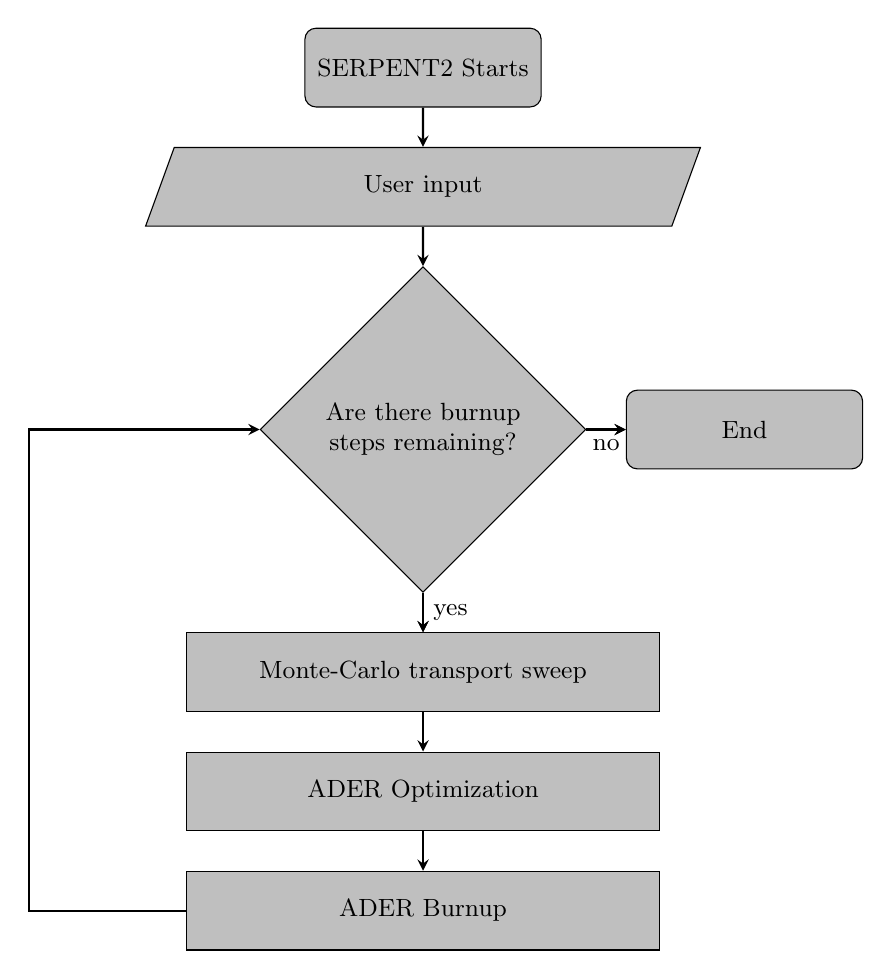
\begin{tikzpicture}[node distance = 1.5cm, every text node part/.style={font=\small}]
\node (start) [startstop] {SERPENT2 Starts};
\node (input) [io, below=0.5cm of start] {User input};
\node (dec1) [decision, below=0.5cm of input] {Are there burnup steps remaining?};
\node (first) [process, below=0.5cm of dec1] {Monte-Carlo transport sweep};
\node (end) [startstop, right=0.5cm of dec1] {End};
\node (ader_opt) [process, below=0.5cm of first] {ADER Optimization};
\node (ader_burn) [process, below=0.5cm of ader_opt] {ADER Burnup};

\draw [arrow] (start) -- (input);
\draw [arrow] (input) -- (dec1);
\draw [arrow] (dec1) -- (first);
\draw [arrow] (dec1) -- node[anchor=west] {yes} (first);
\draw [arrow] (dec1) -- (end);
\draw [arrow] (dec1) -- node[anchor=north] {no} (end);
\draw [arrow] (first) -- (ader_opt);
\draw [arrow] (ader_opt) -- (ader_burn);
\draw [arrow] (ader_burn) -- ([shift={(-2cm,0cm)}]ader_burn.west) |- ([shift={(-2cm,0cm)}]dec1.west) -- (dec1);
\end{tikzpicture}
\end{centering}
\end{figure}

\begin{figure}\label{fig:flowchart2}
\caption{A detailed look of the ``ADER Optimization" box from figure
\ref{fig:flowchart1}. This diagram picks up at the entry to the ``ADER
Optimization" box and exits out to the ``ADER Burnup" box also in figure
\ref{fig:flowchart1}.}
\begin{centering}
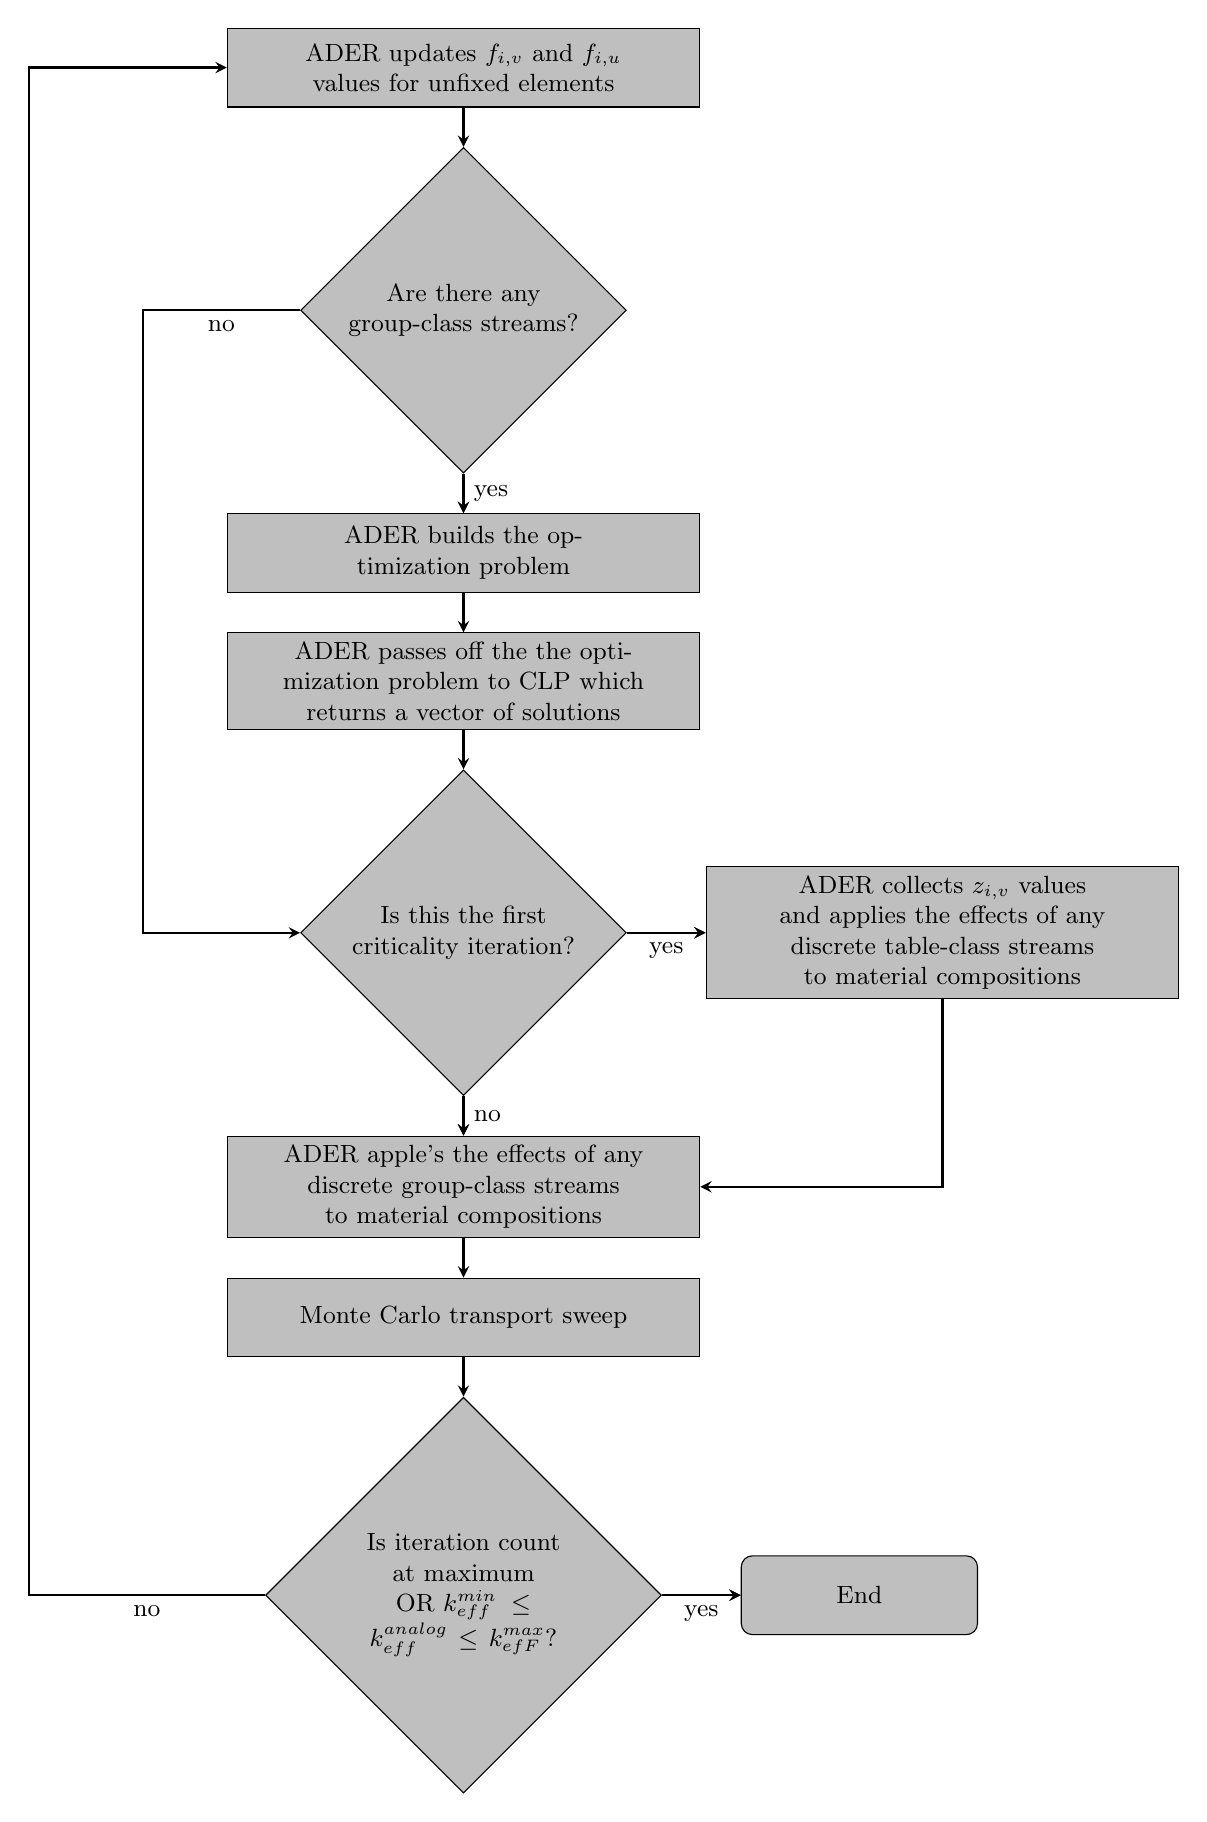
\begin{tikzpicture}[node distance = 1.5cm, every text node part/.style={font=\small}]
\node (ader_gather) [process] {ADER updates $f_{i,v}$ and $f_{i,u}$ values for 
unfixed elements};
\node (dec1) [decision, below=0.5cm of ader_gather] {Are there any group-class
streams?};
\node (ader_build) [process, below=0.5cm of dec1] {ADER builds the
optimization problem};
\node (clp) [process, below=0.5cm of ader_build] {ADER passes off the the
optimization problem to CLP which returns a vector of solutions};
\node (dec2) [decision, below=0.5cm of clp] {Is this the first criticality 
iteration?};
\node (rem) [process, right=1cm of dec2] {ADER collects $z_{i,v}$ values  and 
applies the effects of any discrete table-class streams to material 
compositions};
\node (ader_apply) [process, below=0.5cm of dec2] {ADER apple's the effects of
any discrete group-class streams to material compositions};
\node (monte) [process, below=0.5cm of ader_apply] {Monte Carlo transport 
sweep};
\node (dec3) [decision, below=0.5cm of monte] {Is iteration count at maximum
OR $k_{eff}^{min} \leq k_{eff}^{analog} \leq k_{efF}^{max}$?};
\node (end) [startstop, right=1cm of dec3] {End};

\draw [arrow] (ader_gather) -- (dec1);
\draw [arrow] (dec1) -- (ader_build);
\draw [arrow] (dec1) -- node[anchor=west] {yes} (ader_build);
\draw [arrow] (dec1) -- node[anchor=north] {no} ([shift={(-2cm,0cm)}]dec1.west) |- ([shift={(-2cm,0cm)}]dec2.west) -- (dec2);
\draw [arrow] (ader_build) -- (clp);
\draw [arrow] (clp) -- (dec2);
\draw [arrow] (dec2) -- (ader_apply);
\draw [arrow] (dec2) -- node[anchor=west] {no} (ader_apply);
\draw [arrow] (dec2) -- (rem);
\draw [arrow] (dec2) -- node[anchor=north] {yes} (rem);
\draw [arrow] (rem) -- (rem.south) |- ([shift={(1cm,0cm)}]ader_apply.east) -- (ader_apply);
\draw [arrow] (ader_apply) -- (monte);
\draw [arrow] (monte) -- (dec3);
\draw [arrow] (dec3) -- (end);
\draw [arrow] (dec3) -- node[anchor=north] {yes} (end);
\draw [arrow] (dec3) -- node[anchor=north] {no} ([shift={(-3cm,0cm)}]dec3.west) |- ([shift={(-2cm,0cm)}]ader_gather.west) -- (ader_gather);
\end{tikzpicture}
\end{centering}
\end{figure}

In a SERPENT2 burnup simulation, following the initial Monte Carlo transport
sweep done at the beginning of every burnup step, ADER enters its criticality
search iterations - even if a criticality search has not been asked for. The
default values for \texttt{kmin} and \texttt{kmax} will cause the criticality
check to pass regardless.

The first consequential action ADER takes in each iteration is to determine
the $f_{i|e,u}$ and $f_{i|e,v}$ values for the isotopes of unfixed elements
in groups and group-class streams. Following this assessment all of the
$z_{i,v}$ values are calculated for table-class streams.

This point marks the first major divergence of any ADER simulation.
\textit{If and only if} the only streams entered by the user are table-class
streams the simulation proceeds to the application of the effects of discrete
form streams. There is no optimization process in this case because the user 
has only given direct orders to ADER in the form of table-class streams, there 
are no choices for ADER to make in the form of group-class streams. 

In the case that at least one group-class stream, attached to a material, exists
in the simulation, the simulation would then proceed to build and solve the
optimization problem for each material cluster.

The CLP library expects a linear programming matrix from ADER.
Figure \ref{fig:opt_matrix}
depicts the scheme for constructing the linear programming matrix. Column bounds
are presented above the appropriate column whereas row bounds are presented to 
the left of the appropriate row. Below the column bounds are the variables which
the columns represent and to the right of the row bounds are the equation
number, if any, of the equation that row is modeled after. 
For the sake of brevity
the matrix in Figure~\ref{fig:opt_matrix} is for one material only though many
materials may be involved in such a matrix should they be linked together
by shared mass transfers. In which case the only variables shared between 
materials in the same material cluster are the
group-class streams and the stream equations they are a part of are the only
coupling equations; aside from transfers by table-class streams but those
are only represented in the linear programming matrix, they are handled by
other routines all together. If a second material were to be included in this
matrix then, perhaps, the stream entries in the fourth, fifth, and sixth 
columns would have non-zero coefficients for some $E_{j}^{d}$ and $I_{k}^{d}$ 
rows of the second material. The coefficients used for the construction of these
matrices are normalized to the atomic density from the beginning of the
optimization process for the host material.

Working down the matrix row by row the first row encountered represents
equation \ref{eq:rto_min} with arbitrary groups $g_{1}$ and $g_{2}$ whereas 
the next row 
down represents equation \ref{eq:rto_max}. The third row, what will be referred
to as an elemental future row represents the atom balance for element $j$ where
$f{e_{j}^{u}}$ is the fractional proportion of element $j$ in group $u$.
The novel column involved here is an elemental future column whose inclusion
in the same row closes the equation where an ``elemental future value",
$E_{j}^{f}$, is the fraction of a material's atomic density ( relative to
the density at the beginning of the step ) that is taken up by element $e_{j}$.
The bounds for this row are those for a
free element, a concept covered in section \ref{ssec:control}, 
those elements which are permitted to have portions
of the element not tied up in declared group structures. In the case of a
controlled element, those who's complete abundance must be accounted for by
group structures, the lower bound is changed to zero. 
The fourth row, an elemental
delta row, represents the change in the abundance of element $j$,
$E_{j}^{d}$, as caused by all group-class streams where
$f{e_{j}^{v}}$ is the fractional proportion of element $j$ in stream $v$. 
Of course the elemental delta column 
is involved to close the balance. The fifth row, or balance row, is what ties
together $E_{j}^{f}$ and $E_{j}^{d}$. The bounds, $\alpha$ and $\beta$,
are equal and represent $E_{j}^{c} + r_{e_{j}}$ constituting an element 
balance ``in time” where $E_{j}^{c}$ represents the present fractional
abundance of element $j$. The fifth row requires, straightforwardly, that the
future amount of an element be equal to the current amount plus any delta,
or change, in the element's abundance. The sixth row is an isotopic balance row
requiring that the abundance of an element be equal to the abundance of its
constituent isotopes. 
The following three rows, the seventh, eighth, and ninth,
are the isotopic versions of the elemental future, delta, and balance rows 
where $f$ values are for the isotopic fractional proportions.
$\gamma$ and $\delta$ are
equal and represent $I_{k}^{c} + r_{i}$ where $I_{k}^{c}$ represents
the present fractional abundance of isotope $k$. In the tenth and eleventh rows
Equations \ref{eq:k_max} and \ref{eq:k_min} find representation with $\eta$
and $\theta$ respectively representing terms of the expanded sum found in the
referenced equations; $\frac{k_{eff}^{min}}{P_{A}} \sigma_{a}^{k} - \nu^{k}
\sigma_{f}^{k}$ and
$\frac{k_{eff}^{max}}{P_{A}} \sigma_{a}^{k} - \nu^{k}
\sigma_{f}^{k}$. 
The twelfth row represents equation \ref{eq:oxi_mb}, accounting for the
contributions of the future quantity of an element to a material's averaged
oxidation state (or however the weighted sum is interpreted).
The thirteenth row, or Pres row, exists
when the user instructs ADER to balance inflows with outflows as discussed
in section \ref{ssec:pres}. The
pres row requires that the net stream transfers in a material come to zero. The
effects of table-class streams are captured in $\upsilon$ and $\omega$ as seen
in equation \ref{eq:upsilon_bound}.
The fourteenth row represents a closure for a group defined with method D from
section \ref{sec:groups}; a summation group. In this case the summation group
is $g_{3}$ which was defined as follows\ldots

\begin{li}
grp g3 sum
g1  w1 
g2  w2
\end{li}

The fifteenth row represents a closure relationship for a summation stream,
a group-class stream built using a summation group. In this case the summation
stream is $s_{3}$.
The final row is the optimization, or Opt row. This row
indicates to the simplex routine which variables to minimize or maximize. In
figure \ref{fig:opt_matrix} the opt row is indicating that $g_{1}$ is the
optimization target.

\begin{equation}\label{eq:upsilon_bound}
\upsilon = \omega = \sum_{i}^{I} r_{i}
\end{equation}

    \begin{equation*}
    \label{fig:opt_matrix}
        \centering
        \begin{blockarray}{cccccccccccc}
                               &                   & [b_{m},b_{M}]  &[0, \infty)
           &[0, \infty)        &[0,\infty)         & [0,\infty)     &[0, \infty)
           &[0, \infty)        &(-\infty,\infty)         & [0,\infty)     &
            (-\infty0,\infty)  \\ 
                               &                   & g_{1}          &g_{2}
            &g_{3}             & s_{1}             & s_{2}          &s_{3}
            &E_{j}^{f}         & E_{j}^{d}         & I_{k}^{f}      &
            I_{k}^{d} \\
                               &                   &                &
            &                  &                   &                &
            &                  &                   &                &
             \\ 
            \begin{block}{cc[cccccccccc]}
             {(-\infty,0]}     & \text{Eq.}\ref{eq:rto_min} & -1    &r_{m}
            &                  &                   &                &
            &                  &                   &                &
             \\
             {[0,\infty)}      & \text{Eq.}\ref{eq:rto_max} & -1    &r_{M}
            &                  &                   &                &
            &                  &                   &                &
             \\
             {(-\infty,0]}     & E_{j}^{f}         & f_{e_{j}^{1}}  &f_{e_{j}^{2}}
            &                  &                   &                   &
            &-1                &                   &                   &
             \\
            {[0,0]}            & E_{j}^{d}         &                   &
            &                  & f_{e_{j}^{1}}     & f_{e_{j}^{2}}     &
            &                  & -1                &                   &
             \\
            {[\alpha, \beta]} 
                               & E_{j}^{b}         &                   &
            &                  &                   &                   &
            &1                 & -1                &                   &
             \\
            {[0,0]}            & E_{j}^{i}         &                   &
            &                  &                   &                   &
            &-1                &                   & 1                 &
             \\
            {(-\infty,0]}      & I_{k}^{f}         & f_{i_{k}^{1}} &f_{i_{k}^{2}}
            &                  &                   &                   &
            &                  &                   & -1                &
             \\
            {[0,0]}            & I_{k}^{d}         &                   &
            &                  & f_{i_{k}^{1}}     & f_{i_{k}^{2}}     &
            &                  &                   &                   &
            -1 \\
            {[\gamma, \delta]}
                               & I_{k}^{b}         &                   &
            &                  &                   &                   &
            &                  &                   & 1                 &
            -1 \\ 
            {[0, \infty)}      & \text{Eq.}\ref{eq:k_max}&             &
            &                  &                   &                   &
            &                  &                   & \eta              &
             \\
            {(-\infty, 0]}     & \text{Eq.}\ref{eq:k_min} &            &
            &                  &                   &                   &
            &                  &                   & \theta            & 
             \\
            {[O_{m},O_{M}]}    & \text{Eq.}\ref{eq:oxi_mb} &           &
            &                  &                   &                   &
            &v_{e}w_{e}        &                   &                   &
             \\
            {[\upsilon,\omega]} & \text{Pres}      &                   &
            &                  & 1                 & 1                 &
            &                  &                   &                   &
             \\
             {[0,0]}           & \text{Eq.}\ref{eq:t_group_sum} & -w_{1|3} &-w_{2|3}
            &1                 &                   &                &
            &                  &                   &                &
             \\
             {[0,0]}           & \text{Eq.}\ref{eq:t_streams_sum} &  &
            &                  &-q_{1|3}           &-q_{2|3}        &1
            &                 &                   &                &
             \\
                               & \text{Opt}        & 1                 &
            &                  &                   &                   &
            &                  &                   &                   &
             \\
            \end{block}
        \end{blockarray}
    \end{equation*}

\subsection{Solving the Optimization Problem}\label{ssec:clp}
Once the matrix seen in figure \ref{fig:opt_matrix} has been constructed by ADER
it is converted into a dense column-major format and passed off to the CLP 
library which solves this matrix as a simplex problem. CLP then returns a
vector containing the atomic density of each group in a material, normalized to
the material's density at the beginning of the optimization process. This
vector also contains all the group-class mass load values needed to bring
the material cluster to the optimal state. If the simulation is in the first
criticality search iteration for a burnup step, the actions of all discrete 
form streams,both group-class and table-class, are applied to materials. If the
simulation is past the first criticality search iteration for the current
burnup step only the actions of discrete group-class streams are applied to
materials. Following these actions a Monte Carlo transport sweep is run with
all the same cycle and batch parameters as specified by the user in the
SERPENT2 input files. At this point, if the system $k_{eff}^{analog}$ is within
the bounds as set by the user (or the default bounds) or if the criticality
search has already used up all of its iterations, the simulation progresses
on to the burnup calculation. If not, another criticality search iteration is
launched starting with the determination of the isotopic composition for
all unfixed elements in groups and group-class streams.

\subsection{Nuclear Burnup Calculations}\label{ssec:burn}
ADER's burnup routine rides along the iteration scheme employed by the SERPENT2
burnup routine. That is to say that ADER is compatible with any burnup
correction scheme that the user employs through SEREPNT2. In truth, the only
affect that a burnup iteration scheme has on ADER is to change the cross
sections used in any criticality control rows in the optimization matrices.
ADER extends the burnup capabilities of SERPENT2 to include the effects
of both group and table-class streams.
The coefficients in the burnup
matrix are those from the Bateman equation as seen in equation
\ref{eq:Bateman} for the one energy group and zero 
dimensionality case, where $N$ is the number density of nuclide $n$,
$t$ is time, $b_{m \to n}$ is the branching ratio for the decay of 
nuclide $m$ into $n$, $\lambda$ is the decay constant
for its sub-scripted nuclide,
$q$ goes over all neutron induced absorption reactions for a given isotope, 
$a_{m \to n}^{q}$ is the branching ratio for isotope $m$ into $n$ due to
reaction $q$, $\sigma_{x}^{y}$ is the effective microscopic
cross section of reaction $x$ for isotope $y$, $\phi$ is the
scalar neutron flux, $d$ denotes all
transmutation reactions for a given isotope, $R_{n}(t)$ is a
fractional removal (or addition) rate for isotope $n$ at
time $t$, and $F_{n}(t)$ is a feed (or removal) amount for isotope
$n$ at time $t$. These last two terms in equation \ref{eq:Bateman}
account for proportional and continuous form streams
respectively.

A highly truncated burnup scheme can be
seen in figure \ref{fig:burn_matrix} in which there are two isotopes,
\ce{^{233}U} and \ce{^{135}Xe}, and two streams; $S_{c}$ representing a
continuous stream with a constant injection rate and $S_{p}$ representing a
proportional stream with a transfer rate dependent upon the concentration
of the substances to be transferred. There are, of course, two matrices as well.
The burnup matrix to the left holding the coefficients of the Bateman equation
and the second, to the right, holding the initial concentrations of isotopes
and the values for the streams. The first column of the first row gives
the creation and destruction of \ce{^{233}U} which is dependant on the
concentration of \ce{^{233}U} with $\Gamma$ representing nuclear destruction as
seen in equation \ref{eq:Gamma_def}. The third column of the first row holds
the fraction of stream $S_{c}$ that \ce{^{233}U} comprises. These entries
together describe the evolution of \ce{^{233}U} in the given system. In the
second row $\Xi$, as seen in equation \ref{eq:Xi_def}, represents the production
of \ce{^{135}Xe} from \ce{^{233}U}. In the second column of the second row are
the processes dependant on the concentration of \ce{^{135}Xe}. $\Upsilon$
represents the proportional rate constant as determined by the multiplication
of $q_{i,v}$ and $r_{v}$ whereas $\Theta$ is given by equation 
\ref{eq:Theta_def}. The third row is blank as the abundance of a continuous type
stream, $c_{n}$, does not change over a burn step. The fourth row is an
addition specific to ADER and not found in the Bateman equations; rather, this
line, and the lines it represents, exists to keep track of the amount of an
isotope that a proportional stream moves simply to provide this information
to the user. The system of matrices seen in figure \ref{fig:burn_matrix} is
solved by SERPENT2 using the CRAM methodology providing updated isotopic
abundances and proportional stream transfer amounts.

    \begin{equation}
    \label{eq:Bateman}
    \begin{split}
        \frac{\mathrm{d}N_{n}(t)}{\mathrm{d}t} = & \sum \limits_{m}^{M} 
        b_{m \rightarrow n} \lambda_{j} N_{j}(t) + \\
        & \sum \limits_{m}^{M}
        \sum \limits_{q}^{Q} a_{m \rightarrow n}^{q}
        \sigma_{q}^{k} \phi(t) N_{k}(t) - \\
        & N_{n}(t) \lambda_{i} - \sum \limits_{d}^{D}
        \sigma_{d}^{n} \phi(t) N_{n}(t) - \\
        & R_{n}(t) N_{n}(t) + F_{n}(t)
    \end{split}
    \end{equation}

    \begin{equation}
    \label{fig:burn_matrix}
        \begin{blockarray}{cccccc}
             &
            \ce{^{233}U} &
            \ce{^{135}Xe} &
            S_{c} &
            S_{p} &
            \mathbb{N} \\
             &
             &
             &
             &
             &
             \\ 
        \begin{block}{c[cccc][c]}
            \ce{^{233}U} &
            -\lambda_{\ce{^{233}U}} + \Gamma &
             &
            f^{S_{c}}_{\ce{^{233}U}} &
             &
            N_{\ce{^{233}U}} \\
            \ce{^{135}Xe} &
            \Xi &
            -\lambda_{\ce{^{135}Xe}} + \Upsilon + \Theta &
             &
             &
            N_{\ce{^{135}Xe}} \\
            S_{c} &
             &
             &
             &
             &
            c_{n}\\
            S_{p} &
             &
             \Upsilon &
             &
             &
             0\\
        \end{block}
        \end{blockarray}
    \end{equation}

\begin{equation}
\label{eq:Gamma_def}
\Gamma = - \sum \limits_{d}^{D} \sigma_{d}^{\ce{^{233}U}} \phi
\end{equation}

\begin{equation}
\label{eq:Xi_def}
\Xi = b_{\ce{^{233}U} \rightarrow \ce{^{135}Xe}} \lambda_{\ce{^{233}U}} + \sum
\limits_{q}^{Q} a_{\ce{^{233}U} \rightarrow \ce{^{135}Xe}} \sigma_{q}^{
\ce{^{233}U}} \phi
\end{equation}

\begin{equation}
\label{eq:Theta_def}
\Theta =-\sum \limits_{d}^{D} \sigma_{d}^{\ce{^{135}Xe}} \phi
\end{equation}

Following the solution of the burnup problem the material compositions are
updated accordingly and the simulation moves on to the next burnup step.



\section{Installation}\label{sec:install}
Installing ADER is a five step process: Downloading ADER covered in section
\ref{ssec:dader}, installing the CLP libraries covered
in section \ref{ssec:dclp}, editing the necessary lines in the SERPENT2
base code covered in section \ref{ssec:edit}, compiling the code covered
in section \ref{ssec:compile}, and testing the code, already covered in
section \ref{sec:test}. These instructions assume the user is operating
inside of a linux-like environment.

\subsection{Downloading ADER}\label{ssec:dader}
ADER is available as a public repository hosted at\ldots
\begin{lstlisting}
some_web_address
\end{lstlisting}

Download ADER using your preferred client. The directories contained in the ADER
parent directory, call this folder \texttt{ADER\_Dir}, are\ldots

\begin{itemize}
\item{\texttt{docs} - where this user manual and the API can be found in the
subdirectories \texttt{docs/UM} and \texttt{docs/API}, respectively.}
\item{\texttt{inputs} - where in the subdirectory, \texttt{inputs/Test\_Input},
the file \texttt{test\_input.txt} can be found.}
\item{\texttt{src} - where all of ADER's source files can be found.}
\item{\texttt{System\_Testing} - where all of ADER's system tests can be found
in their respective subdirectories titled after the test which they contain.
Inside of each subdirectory is the test input file and a README file explaining
the operation of the test.}
\end{itemize}

\subsection{Downloading and Installing CLP}\label{ssec:dclp}
CLP is available as a public repository hosted at\ldots

\begin{lstlisting}
https://github.com/coin-or/Clp
\end{lstlisting}

Download CLP using your preferred client. Inside this directory, call it
\texttt{Clp\_Dir}, there is one important subdirectory, \texttt{Clp\_Dir/Clp}.
Inside of this subdirectory executing the following commands in a linux-like
environment should install the Clp libraries on your system\ldots

\begin{li}
./configure
./install-sh
make all
\end{li}

Copy the file \texttt{Clp\_C\_Interface.h}, found in \texttt{Clp\_Dir/Clp/src},
 into your SERPENT2 build directory. 
After this process is complete do not forget to add the path to this
subdirectory to all applicable system paths, most likely just your system
\texttt{PATH}.


\subsection{Editing SERPENT2}\label{ssec:edit}
These instructions assume that the base version of SERPENT2 being modified
is version 2.1.31. ADER DOES NOT WORK WITH VERSIONS OF SERPENT2 EARLIER THAN
2.1.30.
Compatibility with future versions of SERPENT2 and installation directions
are not guaranteed.
To configure SERPENT2 to interact with ADER three steps are necessary. First,
copy all of the files found in \texttt{ADER\_Dir/src}, to the SERPENT2
\texttt{src} directory ( or wherever you build SERPENT2).
This might look something like the following\ldots

\begin{li}
cd ~/SERPENT2_Dir
cp ~/ADER_Dir/src/* ./src/
\end{li}

In the directory \texttt{ADER\_Dir/docs/UM} there is a file named 
``Source\_mod.txt". ``Ln" is short for ``line number".
The contents of this file have the following format\ldots

\begin{lstlisting}
[function_name].c: Line number or description of location in file
{
#ADER MOD BEGIN#
contents to add to file at the designated location
#ADER MOD END#
}
\end{lstlisting}

For each listing, add the code contents found between the
\texttt{ADER MOD BEGIN} and \texttt{ADER MOD END} tags to the
actual SERPENT2 source file given at the location
described: this is either inserting new code lines following an existing
SERPENT2 source line given as either an insertion listing or as a single line
number or as a range of line numbers in which case this range is to be fully
replaced by the ADER code sample. 
A suggestion is to execute these file modifications
from the modifications closest to the end of the file to the
modification closest to the beginning of the file - in this way
the line numbers you look for are unchanged by the addition of
the ADER code.
It is considered good practice to include the tags themselves
,\texttt{ADER MOD BEGIN} and \texttt{ADER MOD END}, 
but this is not strictly necessary.
Consider the file, ``main.c", seen below\ldots

\begin{lstlisting}
#include header.h

void main(args)
{
long j;
long i = 0;

i = 1;

return(i);
}
\end{lstlisting}

Now consider that one of the entries in the file
``Source\_mod.txt" looks like the below\ldots

\begin{lstlisting}
Main: Ln 6-8
{
#ADER MOD BEGIN#
for(j=0; j<10; j++)
{
    i++;
}
#ADER MOD END#
}
\end{lstlisting}

The correctly modified main.c file would look like the below where lines 6 
through 8 of the base file were replaced with the content between and including
the ADER mod tags: ``\texttt{ADER MOD BEGIN}" and ``\texttt{ADER MOD END}".
Please use your best discretion when editing these files. If a line number
direction would cut off a \texttt{for} loop and cause compilation or logic
errors, obviously that line number is incorrect and should be slightly
different.

\begin{lstlisting}
#include header.h

void main(args)
{
long i = 0;
#ADER MOD BEGIN#
for(j=0; j<10; j++)
{
    i++;
}
#ADER MOD END#
return(i);
}
\end{lstlisting}

\subsubsection{Modifying the Makefile}\label{sssec:makefile}
Add the following lines to the SERPENT2 Makefile before the \texttt{OBJS} list
but replace \texttt{[absolute/path/to/the/CLP/library]} with the actual path
to the Clp library on your system.

\begin{li}
# ADER MOD BEGIN #
###############################################################################

# Below should be "-L[absolute/path/to/the/CLP/library] -lclpsolver
#     and -L[absolute/path/to/the/CLP/library] -lclp

LDFLAGS += -L/Clp_Dir/Clp/lib -lClpSolver -L/Clp_Dir/Clp/lib -lClp

# Enable ADER_TEST to run the test_input.txt file to execute the 
#     unit and integration test suite

#CFLAGS += -DADER_TEST

# Enable ADER_INT_TEST to ouput the files necessary for integration
#     testing. Many of these files are human readable and useful 
#     for manual debugging

#CFLAGS += -DADER_INT_TEST

# Enable ADER_DIAG to output a copious amount of debugging data

#CFLAGS += -DADER_DIAG

###############################################################################
# ADER MOD END #
\end{li}

In the directory \texttt{ADER\_Dir/docs/UM} there is a file named 
``Object\_list.txt" - add the contents of this file to the SERPENT2 Makefile
\texttt{OBJS} list. You may alphabetize the entires if you care to but it is
not necessary.

In the directory \texttt{ADER\_Dir/docs/UM} there is a file named 
``Build\_list.txt" - add the contents of this file to the SERPENT2 Makefile
build list - the long list of makefile build instructions at the bottom
of the file. You may alphabetize the entries if you care to but it is
not necessary.

\subsection{Compiling ADER}\label{ssec:compile}
To compile ADER with SERPENT2, after having followed the steps in all previous
subsections of this section, give the command below inside of your 
\texttt{SERPENT2\_Dir/src} directory\ldots

\begin{li}
make all
\end{li}

To compile ADER for unit testing, uncomment the line with the phrase
''\texttt{CFLAGS += DADER\_TEST}". When compiled this way the entire code will
work for no other purpose than ADER unit testing conducted with the file
``\texttt{test\_input.txt}" found inside the 
``\texttt{ADER\_Dir/inputs/Test\_Input}" directory.

The compilation flags ``\texttt{DADER\_DIAG}" and ``\texttt{DADER\_INT\_TEST}"
are covered in section \ref{ssec:output_dev}.


\end{document}
